% !TEX root = ..\thesis.tex



\chapter{XÂY DỰNG MÔ HÌNH SERVER XỬ LÝ VÀ HIỂN THỊ DỮ LIỆU RÁC}


\section{Nodejs Server}
\subsection{Giới thiệu tổng quát}
Nodejs là nền tảng phù hợp nhất đối với các ứng dụng nhận và xử lý dữ liệu realtime từ các thiết bị IoT. Vì thế, sử dụng Nodejs Server sẽ hỗ trợ tốt trong quá trình gửi dữ liệu realtime từ The Things Network (TTN) đến server thông qua HTTP và nhận, xử lý dữ liệu nhanh chóng nhờ vào cơ chế và các thư viện, gói mà Nodejs sở hữu. Bên cạnh đó, những thiết bị ảo cũng được lập trình với chức năng gần giống như các thiết bị IoT thật để tăng khả năng mở rộng của dự án khi chỉ có một số lượng nhỏ thiết bị thật cũng như hỗ trợ quá trình kiểm tra lỗi và hiển thị trực quan.

Ngoài việc xử lý nội bộ bên trong, Nodejs còn hỗ trợ kết nối với nhiều server bên thứ ba để tận dụng những API liên quan đến dự án như quản lý, hiển thị, địa lý, tiên đoán, ...

\subsection{Modules và packages được sử dụng}
Nodejs sử dụng kiến trúc Module để đơn giản hóa việc tạo ra các ứng dụng phức tạp, mỗi module chứa một tập các hàm chức năng khác nhau tùy vào mục đích của đối tượng. Bên ngoài những module tích hợp sẵn trong Nodejs, những module bên ngoài có thể được cài đặt vào nhờ vào trình quản lý package của Nodejs (npm). 

\begin{itemize}
    \item Những module tích hợp được sử dụng:
    \begin{itemize}
        \item http: biến server hoạt động như một máy chủ HTTP.
        \item fs: xử lý hệ thống tệp.
        \item os: cung cấp thông tin về hệ điều hành.
        \item cluster: chia nhiều luồng xử lý để tự động phân chia công việc.
    \end{itemize}
    \item Những module bên ngoài được sử dụng:
    \begin{itemize}
        \item dotenv: tải các biến môi trường từ tệp .env vào process.env.
        \item body-parser: phân tích cú pháp các phần thân nội dung yêu cầu đến trong phần mềm trung gian trước trình xử lý.
        \item express: framework được xây dựng trên nền tảng của Nodejs, cung cấp các tính năng mạnh mẽ để phát triển web hoặc mobile.
        \item cors: cơ chế cho phép nhiều tài nguyên khác nhau (fonts, Javascript, v.v…) của một trang web có thể được truy vấn từ domain khác với domain của trang đó.
        \item morgan: log trạng thái HTTP request.
        \item async-waterfall: hỗ trợ chạy một loạt các hàm không đồng bộ nối tiếp nhau, mỗi hàm chuyển kết quả của chúng cho các hàm tiếp theo.
        \item request: thực hiện HTTP request tới các server bên thứ ba.
        \item lodash: thư viện chuyên xử lý logic các nhóm đối tượng.
        \item random: trình tạo số ngẫu nhiên hỗ trợ nhiều phân phối phổ biến.
        \item csvtojson: chuyển đổi tệp .csv thành định dạng json hoặc mảng cột.
        \item moment: thư viện hỗ trợ xử lý thời gian.
        \item csv-write-stream: lưu trữ giá trị vào file csv thông qua luồng mã hóa CSV.
    \end{itemize}
\end{itemize}

Ngoài các module tích hợp và module bên ngoài, chương trình còn có một số module chức năng tự viết để giảm tải tính lặp lại khi lập trình.

\subsection{API}
Nodejs Server là trung tâm xử lý chính luồng dữ liệu gửi đến, cung cấp những một loạt những API liên quan đến khởi tạo thiết bị, cảm biến thật và ảo, nhận và xử lý dữ liệu sau đó lưu vào database. Ngoải ra còn có API gọi tới Python server để xử lý Deep Learning cho những thùng chưa đầy, và API tìm đường đi tối ưu nhất đến các thùng đã đầy hoặc dự đoán sắp đầy.

Sau đây là tất cả API mà server cung cấp với bản mô tả chi tiết từng luồng chức năng:
\begin{itemize}

    \item Xử lý chung:
    \begin{itemize}
        \item POST /api/devices: Tạo và cài đặt thùng rác, cảm biến
        \begin{description}
            \item Mô hình luồng xử lý được mô tả tổng quát ở hình \ref{fig:create_device} 
        \end{description}
        \begin{itemize}
            \begin{figure}[H]
                \centering
                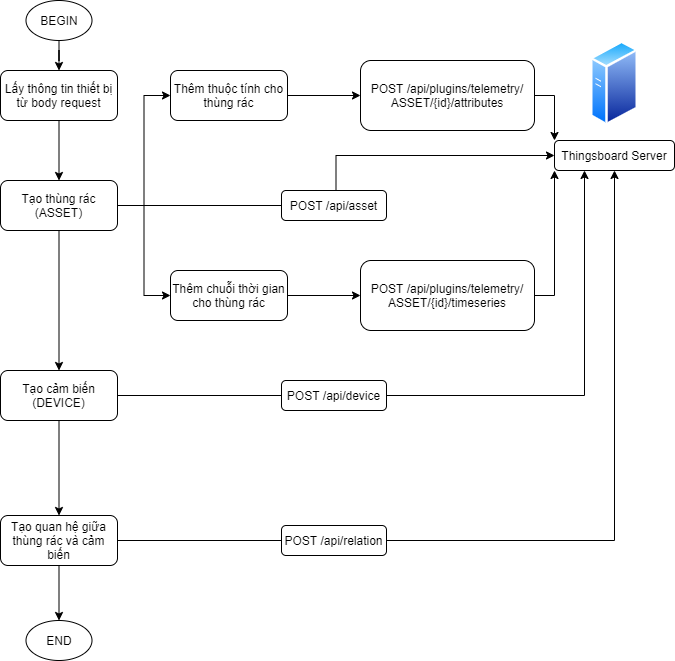
\includegraphics[width=\textwidth]{images/Khanh/Nodejs/Server_Create_Stimulate_Device.png}
                \caption{Sơ đồ miêu tả mô hình khởi tao thiết bị và cảm biến}
                \label{fig:create_device}
            \end{figure}
            \item Trước khi tạo một thùng rác thật/ảo mới cũng phải điền đầy đủ những thông tin sau trong body:
            \begin{itemize}
                \item name (string): tên thùng rác.
                \item type (string): loại thùng rác.
                \item address (string): địa chỉ của thùng, nếu không có thì sẽ sử dụng API Geocoding từ Mapbox nhận vào tọa độ của thùng để định vị địa chỉ.
                \item latitude (double): kinh độ.
                \item longitude (double): vĩ độ.
                \item nonrecycleHeight (double): chiều cao ngăn không tái chế.
                \item recycleHeight (double): chiều cao ngăn tái chế. 
            \end{itemize} 
            \item Sau khi gửi body request như trên, một loạt hàm sẽ được chạy dựa trên cơ chế waterfall, sử dụng request để gọi API khởi tạo từ Thingsboard. Những API từ Thingsboard đều có JWT để bảo mật route, khi sử dụng phải cần có token đăng nhập lấy từ API POST /api/auth/log. Token sau đó được gắn vào header ở dạng 'Bearer \{token\}' ở trường 'X-Authorization'. Nếu không có token thì mọi API sẽ trả về status 401 unauthorized.
            \begin{enumerate}
                \item POST /api/asset để tạo mới thùng rác, nhận vào \{name, type\} của thùng rác. Nếu status trả về là 201 tức là tạo thùng rác thành công, còn 404 là báo lỗi trùng tên thùng rác. ID thùng rác trả về sẽ được lưu trữ.
                \item POST /api/device để tạo mới cảm biến, nhận vào \{name, type\} của cảm biến. Vì trong thùng luôn chứa hai cảm biến siêu âm để phân loại rác tái chế và không tái chế nên tên cảm biến sẽ được chuẩn hóa theo dạng '\{name\}{\_}\{function\}', ví dụ: '\{name\}{\_}taiche' và '\{name\}{\_}khongtaiche'. Nếu status trả về 201 tức là tạo cảm biến thành công, còn 404 là báo lỗi trùng tên cảm biến. ID cảm biến trả về sẽ được lưu trữ.
                \item POST /api/plugins/telemetry/ASSET/\{id thùng rác\}/\{attributes || timeseries\} để thêm các thuộc tính hoặc giá trị theo thời gian cho thùng, những thuộc tính mặc định bao gồm \{address, latitude, longitude, recycleHeight, nonrecycleHeight\} còn giá trị thời gian thì có mức rác 2 ngăn, giá trị tiên đoán và message thông báo. Nếu trường đã có thì sẽ thay đổi giá trị trường đó. Nếu status 201 tức là thêm thành công, 404 là báo lỗi thiếu dữ liệu.
                \item POST /api/relation để tạo quan hệ một nhiều giữa thùng rác và cảm biến, nhận vào body dạng \{from: \{type: 'ASSET', id: \{id thùng rác\}\}, to: \{type: 'DEVICE', id: \{id cảm biến\}\}\}. Nếu status 201 tức là thành công, còn 404 là thiếu dữ liệu hoặc id không tồn tại.
                \item Sau khi thao tác thành công, thông tin thùng rác sẽ được lưu lại dưới server để xử lý dữ liệu và dự đoán.
            \end{enumerate}
        \end{itemize}

        \item GET /api/devices/prediction: Xử lý dự đoán mức rác cho những thùng rác chưa đầy, được gọi vào 1 giờ trước khi thu gom rác.
        \begin{description}
            \item Mô hình luồng xử lý được mô tả tổng quát ở hình \ref{fig:predict_empty_bin} 
        \end{description}
        \begin{enumerate}    
            \begin{figure}[H]
                \centering
                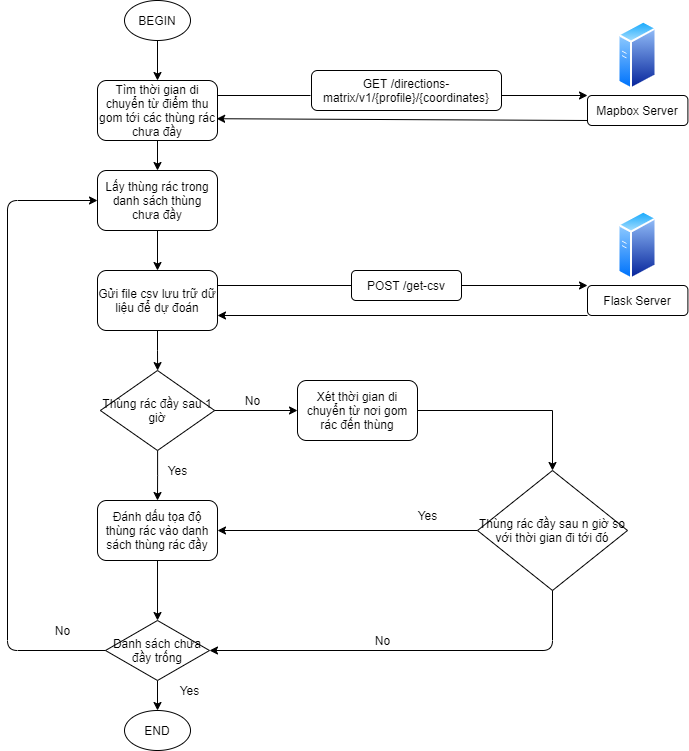
\includegraphics[width=\textwidth]{images/Khanh/Nodejs/Server_Predict_Empty_Bin.png}
                \caption{Sơ đồ miêu tả mô hình gửi dữ liệu tiên đoán và kiểm tra mức rác}
                \label{fig:predict_empty_bin}
            \end{figure}
            \item Lấy tọa độ của những thùng rác chưa đầy, sau đó định dạng theo kiểu chuỗi '\{lng{\_}nơigomrác\},\{lat{\_}nơigomrác\};\{lng{\_}thùng1\},\{lat{\_}thùng1\};\{lng{\_}\newline thùng2\},\{lat{\_}thùng2\} \dots\ '.
            \item Gọi API từ Mapbox GET /directions-matrix/v1/\{profile\}/\{coordinates\}?\newline sources\&annotations\&access{\_}token để lấy ma trận khoảng cách hoặc thời gian di chuyển giữa nhiều điểm. Những params và query được mô tả chi tiết như sau:
            \begin{itemize}
                \item profile (params): cấu hình ID phương tiện, giá trị bao gồm "driving", "walking", "cycling" và "driving-traffic". 
                \item coordinates (params): danh sách tọa độ \{kinh độ, vĩ độ\} được phân tách bằng dấu chấm phẩy.
                \item sources (query): đánh chỉ tọa độ làm điểm nguồn tới tất cả tọa độ còn lại. 
                \item annotations (query): dùng để chỉ định kết quả trả về, giá có thể có là "duration" (thời lượng) hoặc "distance" (khoảng cách) hoặc cả hai ngăn cách bằng dấu phẩy.
                \item access{\_}token (query): token key được cung cấp bởi Mapbox
            \end{itemize}
            \item Kết quả trả về sẽ theo dạng ma trận 1xn (n là số thùng chưa đầy) [0, n1, n2, n3, ...], mỗi phần tử là thời gian di chuyển từ điểm nguồn tới từng tọa độ trong \{coordinates\}.
            \item Duyệt qua những thùng rác chưa đầy, khi file .csv lưu trữ dữ liệu quá ít thì sẽ không dự đoán, còn lại thì sẽ gửi file .csv qua Python Server để dự đoán mức rác vào một giờ sau (giờ gom rác).
            \item Kết quả trả về là một mảng một chiều, mỗi phần tử là lượng rác được dự đoán sau \{index + 1\} giờ. Nếu phần tử 0 (lượng rác vào lúc thu gom) lớn hơn hoặc bằng 90\% chiều cao thùng tức là thùng đó dự đoán sẽ đầy sau một giờ và sẽ được đánh dấu thùng rác đầy.
            \item Đối với những thùng rác dự đoán chưa đầy vào một giờ, thì ta xét trong thời gian từ lúc bắt đầu tới khi đến được thùng rác, thùng có đầy không. Bằng cách lấy thời gian di chuyển đến thùng đó so với các khoảng giờ i (max=3), nếu thời gian nằm trong khoảng giờ i, thì sẽ lấy lượng rác dự đoán sau i + 1 giờ. 
            \item Lấy kết quả dự đoán so với 90\% của thùng, nếu được dự đoán sẽ đầy thì sẽ được đánh dấu vào những thùng đầy.
        \end{enumerate}

        \item GET /api/devices/static-map
        \begin{description}
            \item Mô hình luồng xử lý được mô tả tổng quát ở hình \ref{fig:get_map} 
        \end{description}
        \begin{enumerate}    
            \begin{figure}[H]
                \centering
                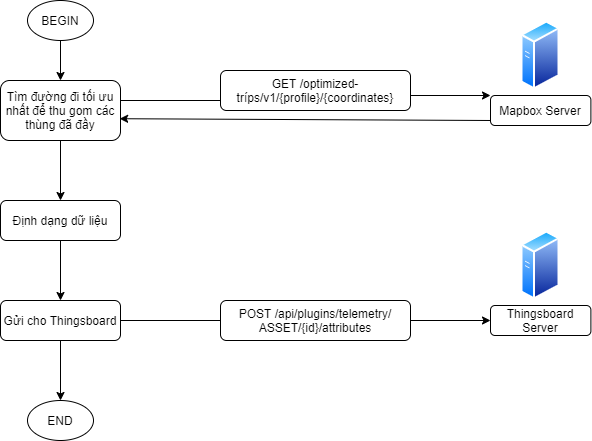
\includegraphics[width=\textwidth]{images/Khanh/Nodejs/Server_Get_Map.png}
                \caption{Sơ đồ miêu tả luồng xuất mảng tọa độ đường đi tối ưu tới thùng rác đầy}
                \label{fig:get_map}
            \end{figure}
            \item Lấy tọa độ của những thùng rác đầy, sau đó định dạng theo kiểu chuỗi '\{lng{\_}nơigomrác\},\{lat{\_}nơigomrác\};\{lng{\_}thùng1\},\{lat{\_}thùng1\};\{lng{\_}\newline thùng2\},\{lat{\_}thùng2\} \dots\ '.
            \item Gọi API từ Mapbox GET /optimized-trips/v1/\{profile\}/\{coordinates\}?\newline language\&roundtrip\&geometries\&steps\&access{\_}token để lấy ma trận khoảng cách hoặc thời gian di chuyển giữa nhiều điểm. Những params và query được mô tả chi tiết như sau:
            \begin{itemize}
                \item profile (params): cấu hình ID phương tiện, giá trị bao gồm "driving", "walking", "cycling" và "driving-traffic". 
                \item coordinates (params): danh sách tọa độ \{kinh độ, vĩ độ\} được phân tách bằng dấu chấm phẩy.
                \item language (query): định dạng ngôn ngữ trả về ở văn bản hướng dẫn.
                \item steps (query): trả về chi dẫn từng chặng chi tiết.
                \item roundtrip (query): cho biết tuyến đường có phải là khứ hồi hay không.
                \item geometries (query): định dạng kiểu trả về, giá trị bao gồm "geojson", "polyline", "polyline6".
                \item access{\_}token (query): token key được cung cấp bởi Mapbox.
            \end{itemize}
            \item Kết quả trả về là một mảng tọa độ chỉ đường đi đến tất cả thùng rác đầy, sau đó định dạng lại theo dạng [[\{lat1\},\{lng1\}],[\{lat2\},\{lng2\}],...].
            \item Gửi kết quả định dạng lên Thingsboard thông qua API POST /api/plugins\newline/telemetry/ASSET/\{id\}/attribute với id của nơi gom rác được tạo sẵn để hiển thị đường đi lên bản đồ Thingsboard.   
        \end{enumerate}
    \end{itemize}

    \item Xử lý dữ liệu cảm biến của thiết bị ảo và thiết bị thật:
    \begin{itemize}  
        \item Mô hình luồng xử lý được mô tả tổng quát ở hình \ref{fig:random_telemetry}
        \begin{figure}[H]
            \centering
            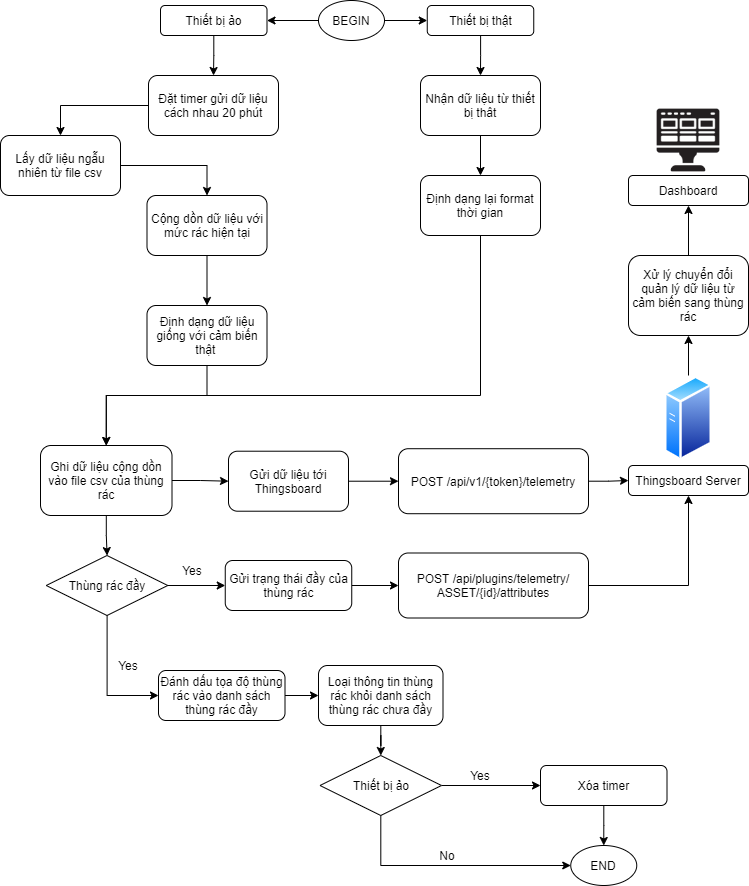
\includegraphics[width=\textwidth]{images/Khanh/Nodejs/Server_Random_Telemetry.png}
            \caption{Sơ đồ miêu tả luồng tạo dữ liệu giả cho thiết bị ảo}
            \label{fig:random_telemetry}
        \end{figure}   
        \begin{enumerate}
            \item Với thiết bị thật (POST /api/TTN/telemetry): 
            \begin{itemize}
                \item Những thiết bị thật sẽ gửi dữ liệu thông qua API này với định dạng là một object được tạo từ TTN được mô tả trong bảng \ref{tab.ttn_format}
                \begin{table}[H]
                    \centering
                    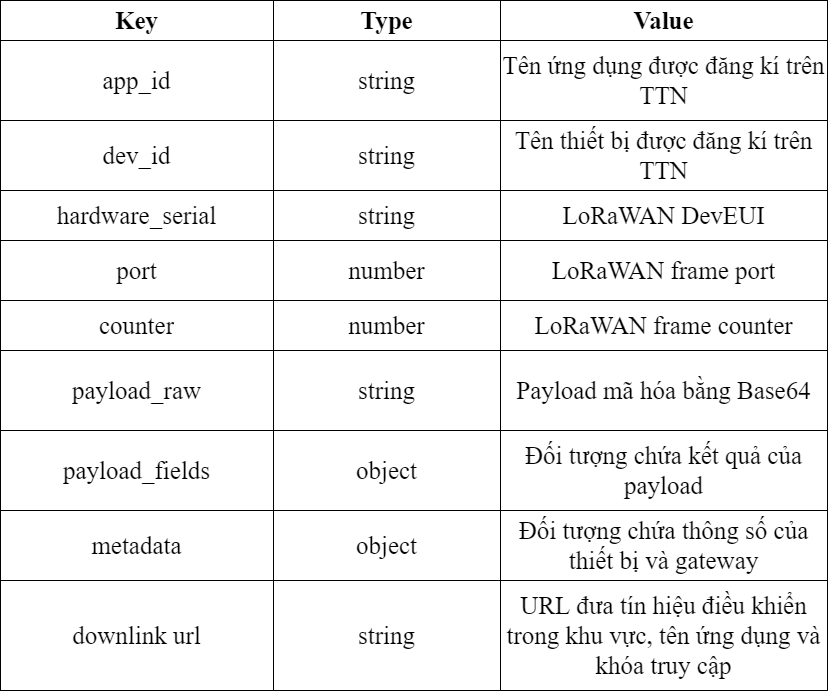
\includegraphics[width=\textwidth]{images/Khanh/Nodejs/TTN_format.png}
                    \caption{Bảng mô tả định dạng dữ liệu được gửi từ TTN}
                    \label{tab.ttn_format}
                \end{table} 
                \item Trong payload\_fields, đối tượng bao gồm tên cảm biến là key và giá trị cảm biến là value (\{ [sensorName]: [sensorValue] \}).
                \item Trong metadata, đối tượng bao gồm các thông số của thiết bị và gateway (tần số, modulation, data\_rate, coding\_rate, ...), nhưng chú trọng nhất là time (thời gian server nhận được gói tin) và tọa độ của thiết bị.
                \item Vì dữ liệu được gửi bằng cảm biến thật nên không cần thay đổi định dạng payload\_fields của chúng, nhưng vì thời gian trong metadata là một chuỗi ISO string, chúng tôi phải định dạng lại kiểu thời gian thành dạng \qq{DD/MM/YYYY hh:mm}, sau đó rồi mới đưa dữ liệu vào file csv.
            \end{itemize}
            \item Với thiết bị ảo (POST /api/devices/\{deviceName\}/random):
            \begin{itemize}
                \item Tiến hành tạo ngẫu nhiên dữ liệu của thùng rác có tên \{deviceName\}, cài đặt timer bằng cách setInterval với khoảng thời gian là 120.000ms (20 phút/1 lần).
                \item Dữ liệu được lấy ngẫu nhiên trong file random.csv với giá trị tái chế và không tái chế ngẫu nhiên từ 0 tới 13.
                \item Khởi tạo mức delta bằng 0, khi thùng rác chưa đầy ta lấy delta cộng với giá trị ngẫu nhiên đó và lấy chiều cao thùng rác trừ cho tổng giá trị sẽ ra được giá trị thật của cảm biến. Thực hiện đến khi nào thùng rác đầy thì giá trị ngẫu nhiên sẽ bằng 0 và khi đó giá trị sẽ dừng ở mức cao nhất của thùng rác.  
                \item Định dạng dữ liệu giống với format payload\_fields của thiết bị thật, đối với thời gian thì sử dụng moment để lấy thời gian thực. 
            \end{itemize}
            \item Sau bước định dạng dữ liệu của 2 loại thiết bị, lưu dữ liệu vào file .csv của từng thùng với tên "\{deviceName\}\_deltaHeight.csv", bên trong file bao gồm các cột timestamp (thời gian), recycleData (dữ liệu tái chế) và nonrecycleData (dữ liệu không tái chế). Đồng thời dữ liệu sẽ được gửi lên Thingsboard, chuyển đổi thực thể và hiển thị lên giao diện theo dạng biểu đồ đường.
            \item Khi thùng rác đã đầy, ta sẽ gửi thông báo đến Thingsboard để hiển thị màu sắc, cùng lúc đó, đánh dấu thùng rác đó vào danh sách các thùng rác đầy và xóa khỏi danh sách các thùng rác chưa đầy. Đối với thiết bị ảo, sẽ dừng timer để giảm tải công việc cho server.
        \end{enumerate}
    \end{itemize}
\end{itemize}

\subsection{Cải thiện hiệu suất với Clustering}
Khi chạy một quá trình của Nodejs, nó sẽ chạy trên một luồng duy nhất (single-thread), việc này có nghĩa là nó chỉ kết nối với một nhân (core) duy nhất trên máy chủ. Vì thế, để sử dụng một cách hiệu quả nhất sức mạnh các máy đa nhân (multi-core), ta sẽ phải chạy nhiều quá trình của Nodejs cùng một lúc. Các quá trình này có thể thực hiện ở ngoài Nodejs nhưng Cluster Module đã hỗ trợ cách thức phân luồng bên trong máy chủ để cải thiện thông lượng (request/s) và cập nhật ứng dụng một cách dễ dàng vì đôi khi một số máy khách cần được phục vụ đồng thời.

Cluster Module cho phép khởi tạo các quy trình con (Workers) chạy đồng thời và chia sẻ cùng một port server. Mỗi Workers được tạo đều có vòng lặp sự kiện, bộ nhớ và phiên bản V8 của riêng nó, sử dụng IPC (Inter-process Communication) để giao tiếp với quy trình cha.

Để sử dụng chúng, ta phải cài đặt cluster trong ứng dụng Nodejs.

\textit{\centerline{var cluster = require(\qq{cluster});}}

Sau đó, điều đầu tiên phải làm là xác định phần nào của đoạn mã dành cho Master Process và phần nào danh cho Workers Process.

\textit{\centerline{if (cluster.isMaster) (...)}}

Nếu là Master Process, ta sẽ lấy số core có sẵn trên hệ thống và lặp lại số core để khởi tạo các Worker Process bằng phương thức fork().

\textit{\centerline{let numCores = require("os").cpus().length;}}

\textit{\centerline{for (let i = 0; i < numCores; i++) \{ cluster.fork(); \}}}

Một cluster module chứa một số sự kiện, hai trong số đó là sự kiện phổ biến liên quan đến thời điểm bắt đầu và kết thúc của Workers, đó là sự kiện \qq{online} và \qq{exit}. Ta gọi 2 sự kiện đó bằng \textit{cluster.on}
\begin{itemize}
    \item Sự kiện \qq{online} được thực hiện khi Workers được phân nhánh và được gán id.
    \item Sự kiện \qq{exit} được thực hiện nếu một Worker Process bị chết, sau đó bắt đầu quy trình mới bằng cách đơn giản là phân nhánh (fork) một quy trình khác.
\end{itemize}

Để đánh giá hiệu suất của Nodejs Server sử dụng Clustering Module khi xử lý một lượng lớn các request đến server, chúng tôi sử dụng loadtest để mô phỏng một số lượng lớn các kết nối đồng thời tới API để có thể đo lường hiệu suất của nó. Chúng tôi sử dụng loadtest vào API /api/devices/staticMap như sau:

\textit{\$ loadtest http://localhost:1111/api/devices/staticMap -n 10000 -c 100}
(với -n là tổng số request và -c là số request đồng thời trong đó)

Đầu tiên khi không sử dụng Clustering Module, chúng tôi được kết quả như hình \ref{fig:nocluster10000}:
\begin{figure}[H]
    \centering
    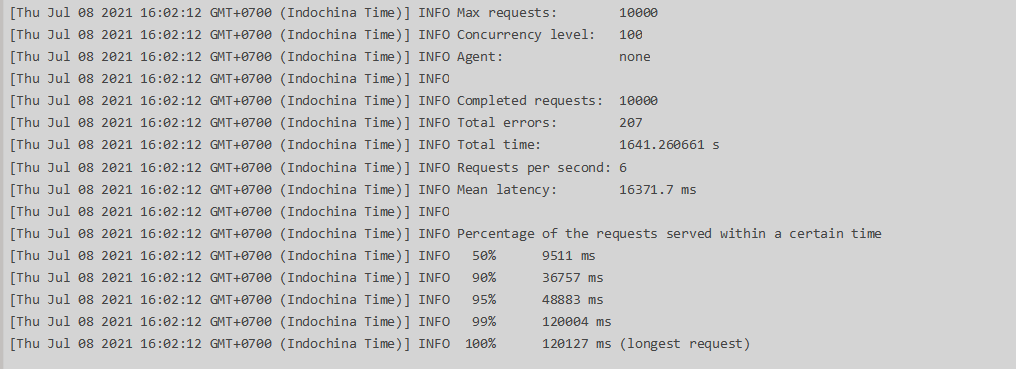
\includegraphics[width=\textwidth]{images/Khanh/Nodejs/NoCluster10000-100.PNG}
    \caption{Hiệu suất của Nodejs khi nhận 10000 request không Clustering}
    \label{fig:nocluster10000}
\end{figure}

Sau đó, khi sử dụng Clustering Module, chúng tôi được kết quả như hình \ref{fig:cluster10000}: 
\begin{figure}[H]
    \centering
    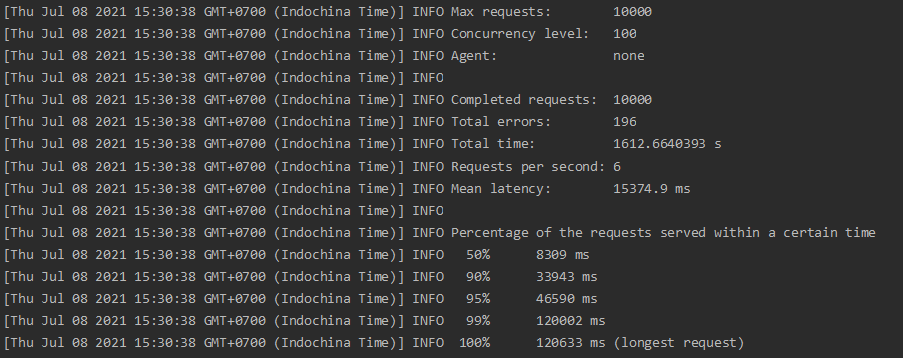
\includegraphics[width=\textwidth]{images/Khanh/Nodejs/WithCluster10000-100.PNG}
    \caption{Hiệu suất của Nodejs khi nhận 10000 request Clustering}
    \label{fig:cluster10000}
\end{figure}

Ta có thể thấy được khi Clustering số request/1 giây là 6 requests, bằng với khi không Clustering, nhưng độ trễ trung bình (mean latency) khi Clustering giảm một chút 15374.9 ms so với 16371.7 ms khi không Clustering.

Sau đó chúng tôi kiểm tra với số lượng request là 100 với request đồng thời là 100 cho API đó, kết quả khi không Clustering như hình \ref{fig:nocluster100} và khi Clustering như hình \ref{fig:cluster100}.

\begin{figure}[H]
    \centering
    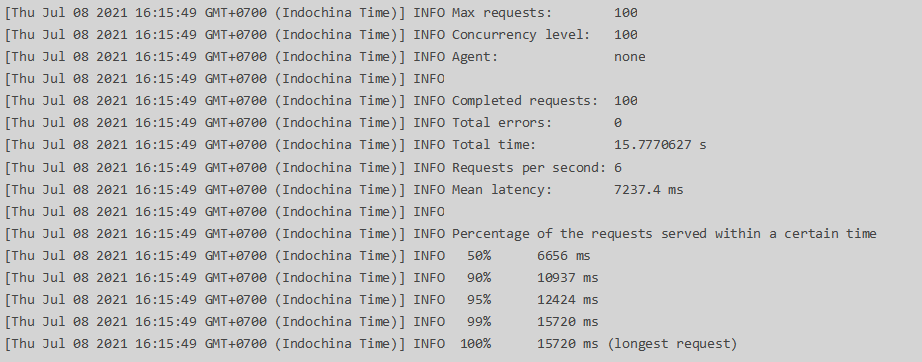
\includegraphics[width=\textwidth]{images/Khanh/Nodejs/NoCluster100-100.PNG}
    \caption{Hiệu suất của Nodejs khi nhận 100 request không Clustering}
    \label{fig:nocluster100}
\end{figure}

\begin{figure}[H]
    \centering
    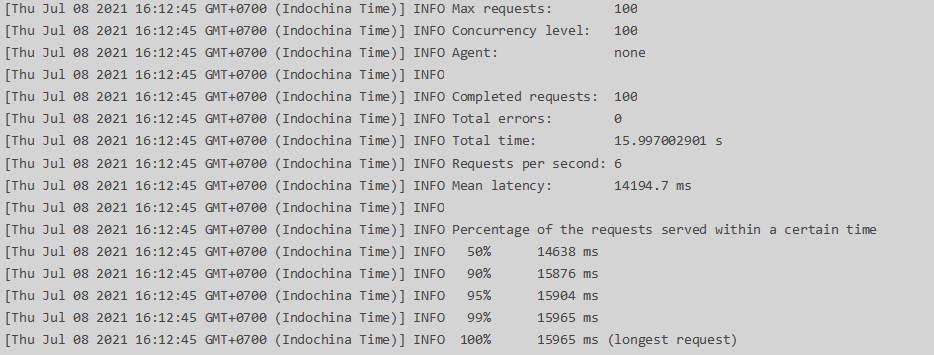
\includegraphics[width=\textwidth]{images/Khanh/Nodejs/WithCluster100-100.PNG}
    \caption{Hiệu suất của Nodejs khi nhận 100 request Clustering}
    \label{fig:cluster100}
\end{figure}

Ở đây lượng request/1 giây của 2 trường hợp đều bằng nhau là 6 request nhưng lần này đối với độ trễ trung bình (mean latency) của trường hợp không Clustering lại nhỏ hơn rất nhiều 7237.4 ms so với khi Clustering 14194.7 ms.

Vì thế, chúng tôi kết luận rằng Cluster Module sẽ hoạt động tốt nhất đối với các thao tác xử lý một số lượng lớn request và trong đó, đoạn mã bao gồm nhiều vòng lặp lớn, tức là nó sẽ tỏa sáng khi liên quan đến các tác vụ đòi hỏi nhiều CPU. Tuy nhiên, nếu ứng dụng không chạy nhiều tác vụ đòi hỏi CPU thì việc tạo ra nhiều Workers sẽ khiến việc phân bổ tài nguyên bổ sung có thể không đáng bởi vì mỗi quy trình đều có bộ nhớ và phiên bản V8 của riêng nó. Vì hiện tại số lượng công việc tại Nodejs Server vẫn chưa đáng kể nên chúng tôi vẫn không khuyến khích sử dụng Clustering, nhưng khi mô hình được mở rộng với nhiều request hơn thì chúng tôi sẽ cân nhắc sử dụng và kiểm tra hiệu suất chính xác.

\section{Python Server}
\subsection{Giới thiệu tổng quát}
Python là sự ưu tiên hàng đầu khi được lựa chọn ngôn ngữ cho các dự án liên quan đến AI. Vì thế sử dụng Python làm một server thứ ba cung cấp API xử lý chính các vấn đề về dự đoán lượng rác, sau đó việc trả kết quả về bên server chính để xử lý tiếp sẽ nhanh và hiệu quả hơn việc xử lý Deep Learning tại Nodejs.

Flask là framework được lựa chọn để xây dựng server vì tính năng hỗ trợ các yêu cầu RESTful và dễ dàng triển khai và tương tác với các server khác. Chức năng chính của server được mô tả tổng quát là cung cấp một API nhận và chuyển một tệp dạng .csv lưu trữ chuỗi thời gian đa biến thành các supervised learning. Sau đó sẽ chia tập lớn thành tập train và tập test, rồi đưa vào mô hình mạng LTSM để dự báo lượng rác sau từng khoảng thời than. 

\subsection{Modules và packages}
Flask có cung cấp thư viện mở rộng flask-restful hỗ trợ cho việc xây dựng các RESTful API một cách nhanh chóng, khuyến khích các phương pháp hay nhất với thiết lập tối thiểu. Ngoài ra, việc xử lý Deep Learning cần sử dụng một số thư viện quan trọng sau:

\begin{itemize}
    \item tensorflow: thư viện mã nguồn mở dùng cho tính toán số học sử dụng đồ thị luồng dữ liệu, xử lý dựa trên sự thay đổi của dữ liệu.
    \item sklearn: thư viện cung cấp một tập các công cụ xử lý các bài toán máy học và mô hình thống kê.
    \item numpy: thư viện lõi của Python, hỗ trợ cho việc tính toán dãy số và ma trận nhiều chiều với tốc độ xử lý nhanh.
    \item math: thư viện hỗ trợ các hàm toán học tiêu chuẩn C.
    \item matplotlib: thư viện hỗ trợ vẽ đồ thị hai chiều, ba chiều mạnh mẽ.
    \item pandas: thư viện hỗ trợ xử lý và phân tích các dữ liệu có cấu trúc (dạng bảng, đa chiều, ...) và dữ liệu chuỗi thời gian nhanh, mạnh mẽ và linh hoạt.
\end{itemize}

\subsection{API}
Server cung cấp 1 API GET /get-csv với luồng dữ liệu được mô tả tổng quát ở hình \ref{fig:python_general}

\begin{figure}[H]
    \centering
    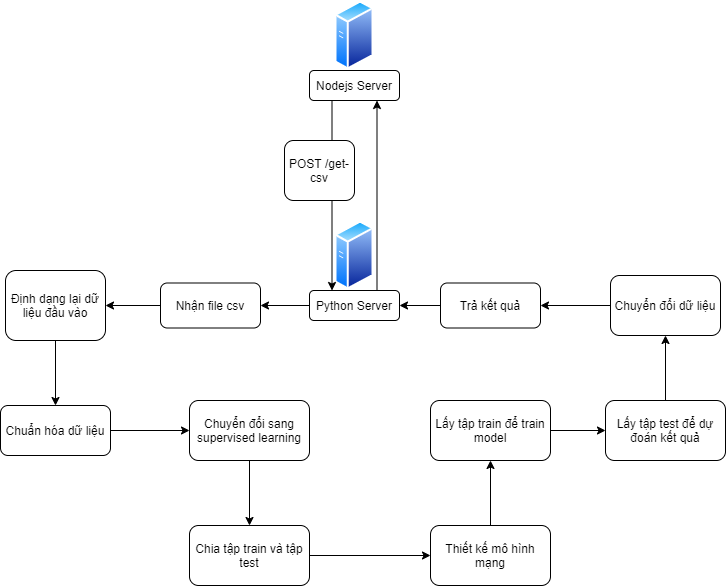
\includegraphics[width=\textwidth]{images/Khanh/Python/Python_general.png}
    \caption{Sơ đồ mô tả tổng quát mô hình Deep Learning dự đoán lượng rác}
    \label{fig:python_general}
\end{figure}

Luồng dữ liệu được mô tả chi tiết như sau:

\begin{enumerate}
    \item Server nhận vào một tệp .csv được gửi từ Nodejs Server, bao gồm các cột [thời gian, lượng rác tái chế, lượng rác không tái chế]. 
    \item Tách riêng 2 cột tái chế và không tái chế thành 2 mảng 2 chiều riêng biệt dưới dạng [[a1],[a2],[a3],...].
    \item Chuyển các mảng thành dạng mảng Numpy và định dạng kiểu float32 để thuận tiện sử dụng.
    \item Chuẩn hóa các mảng bằng MinMaxScaler giúp thuật toán dễ dàng xử lý hơn.
    \item Quy định lấy 75\% chuỗi dữ liệu để làm tập train và phần còn lại để làm tập test. Chuyển đổi tất cả các tập sang supervised learning với số time\_step tự quy định (số time\_step trước đó được sử dụng để dự đoán giá trị ở time\_step tiếp theo).
    \item Kết quả trả về là một mảng 2 chiều có shape là (số lượng dữ liệu, time\_steps). Reshape các tập train input lại thành kiểu (samples, timeseries, features) để đưa vào mô hình dự đoán.
    \item Xây dựng mô hình mạng Stacked LSTM như bảng \ref{tag.lstm.model}
    \begin{table}[H]
        \centering
        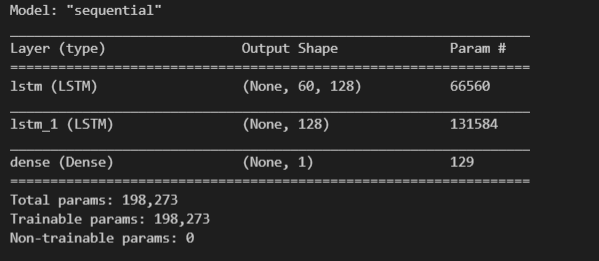
\includegraphics[width=\textwidth]{images/Khanh/Python/LSTM Model.PNG}
        \caption{Tổng quan mô hình mạng LSTM}
        \label{tag.lstm.model}
    \end{table}
    bằng cách tạo một mô hình Sequential và thêm nhiều layer vào trong, cụ thể là 2 LSTM layers và 1 Dense layer với các tham số. Sau đó model sẽ compile với các tham số để train model (loss, optimizer, metrics) và fit data vào để train (bao gồm tổng cộng 198.273 params có thể train được).
    \item Ta lấy \{time\_step\} phần tử cuối từ tập test với t là thời điểm của giá trị cuối cùng để dự đoán dữ liệu ở thời điểm t+1 ... và tiếp đó chạy vòng lặp để dự đoán dữ liệu ở t+2, t+3, t+4 ... bằng cách lấy giá trị dự đoán ở t+1 cho vào mảng, dịch phần tử đầu tiên ra khỏi mảng và tiếp tục dự đoán t+2.
    \item Trả kết quả dự đoán mức rác tái chế và không tái chế về Nodejs Server để tiếp tục xử lý. 
\end{enumerate}

\subsection{Đánh giá dữ liệu}
Chúng tôi gửi một tệp .csv của một thùng rác có chuỗi dữ liệu thu thập mỗi 20 phút vào tháng 6 với tổng 2161 dữ liệu như bảng \ref{tab.CSV_structure}:
\begin{table}[H]
    \centering
    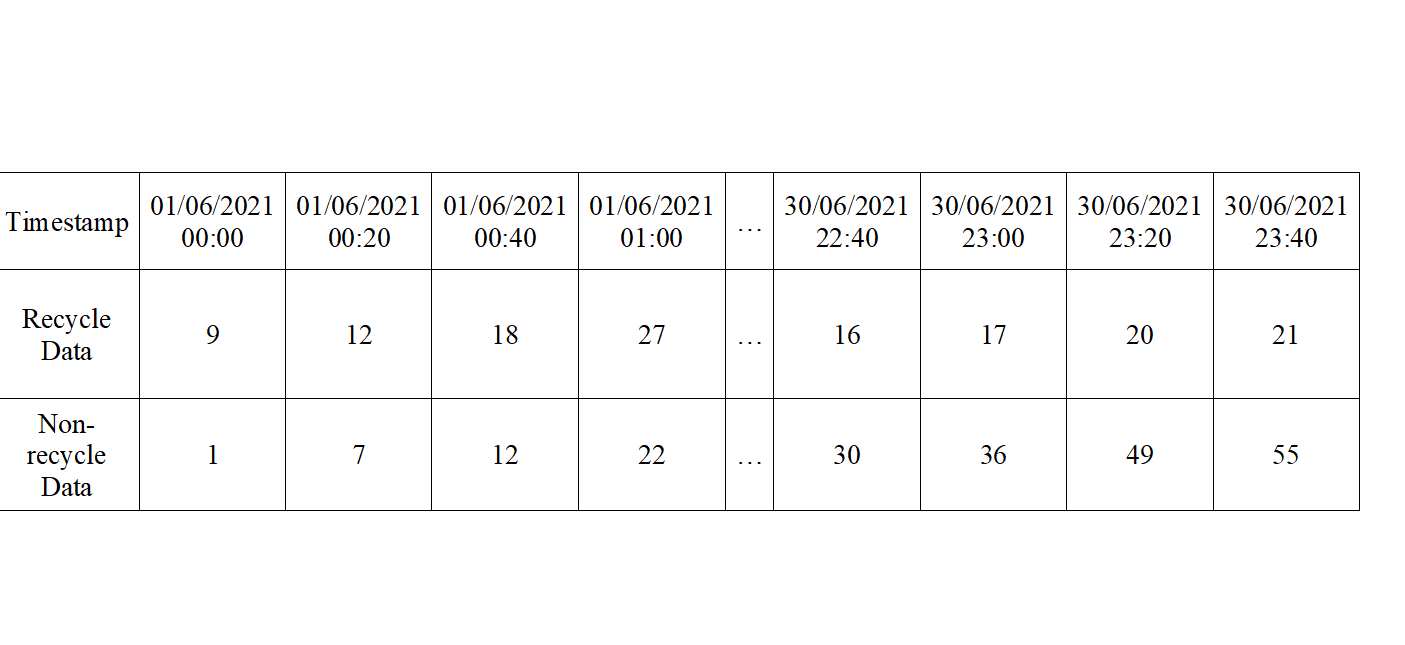
\includegraphics[width=\textwidth]{images/Khanh/Python/CSV_Structure.PNG}
    \caption{Cấu trúc file CSV}
    \label{tab.CSV_structure}
\end{table}

hiển thị dưới dạng biểu đồ hình \ref{fig:CSV_plot_chart}
\begin{figure}[H]
    \centering
    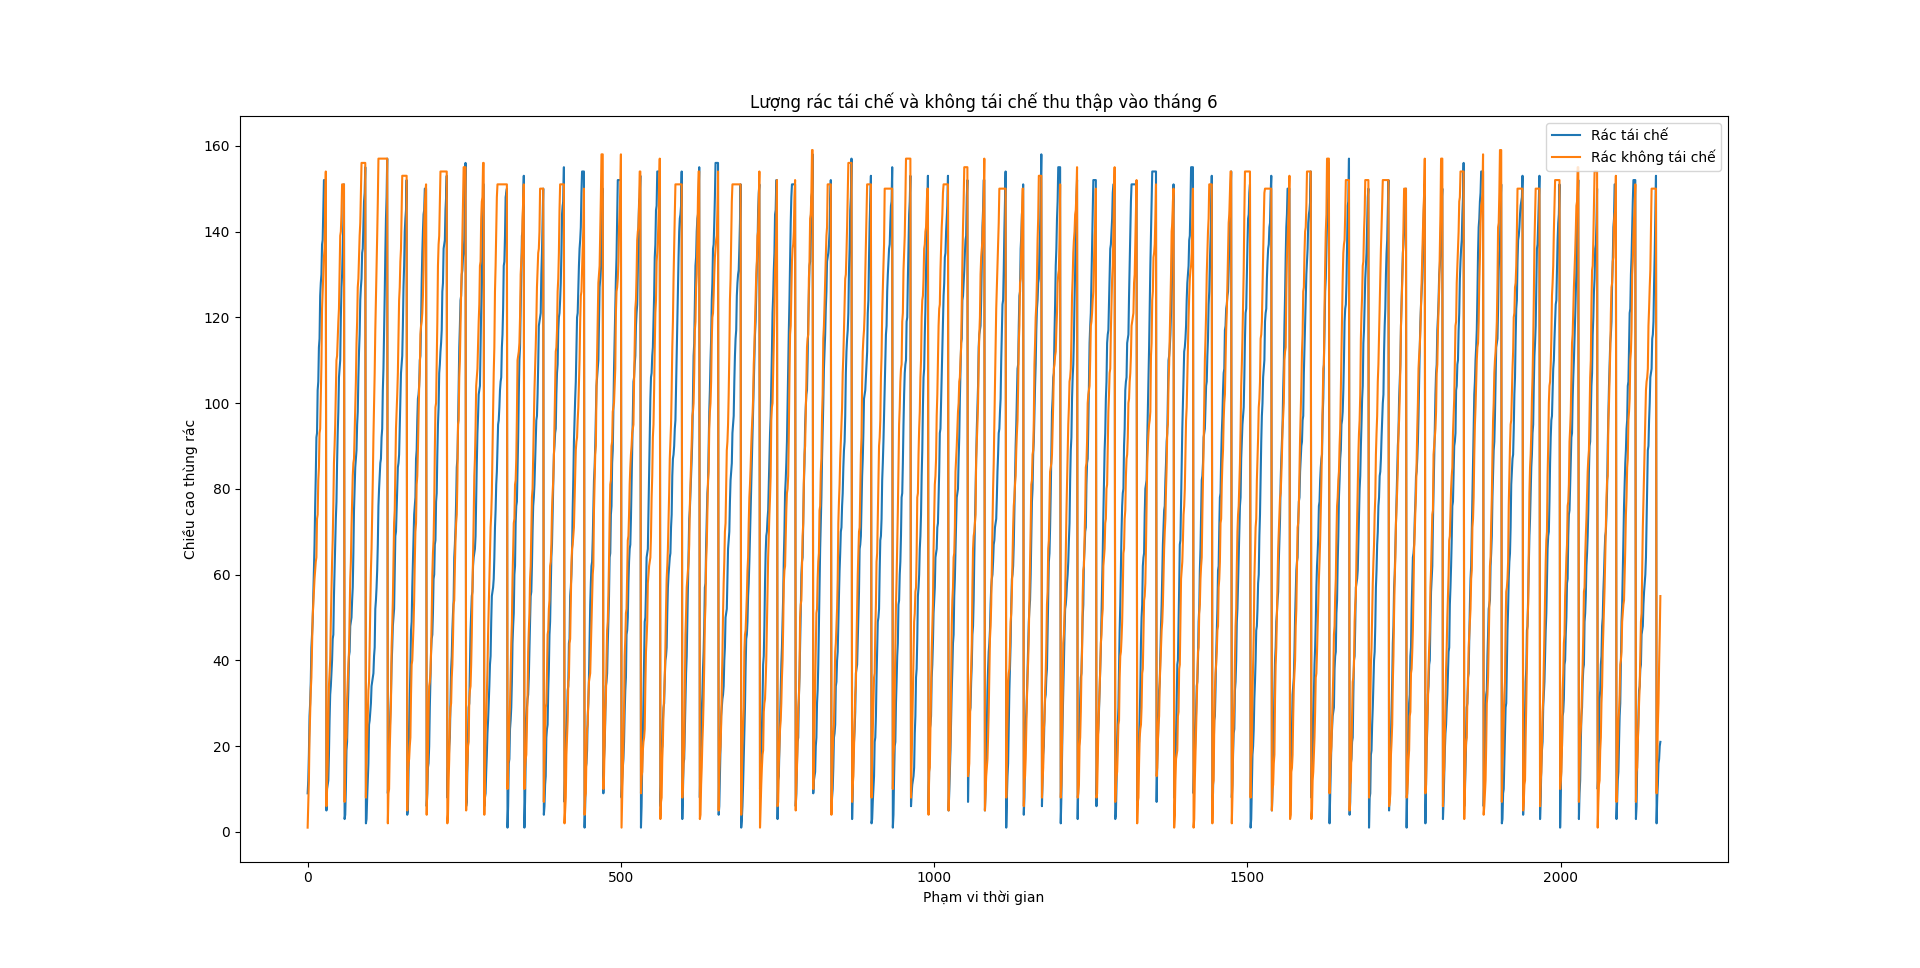
\includegraphics[width=\textwidth]{images/Khanh/Python/CSV_Plot_Chart.png}
    \caption{Biểu đồ lượng rác tái chế và không tái chế thu thập vào tháng 6}
    \label{fig:CSV_plot_chart}
\end{figure}

\begin{description}
    \item timestamp: mốc thời gian
    \item recycle data: lượng rác tái chế
    \item non-recycle data: lượng rác không tái chế
\end{description}

Tập dữ liệu được chuyển thành supervised learning với time\_steps là 60 (tức là lấy dữ liệu 20 tiếng trước để dự đoán) và chia thành 75\% cho tập train (1620) và phần còn lại (541) cho tập test.

Sau khi train mô hình, chúng tôi đánh giá model bằng chỉ số loss để đo tỉ lệ chênh lệch giữa tập dữ liệu thực và tập dữ liệu model dự đoán.

Kết quả train mô hình với 20 epochs cho thấy loss nhỏ nhất trên tập train là 0.05242335423827171 và trên tập test là 0.047845833003520966, được biểu diễn ở biểu đồ \ref{fig:loss_chart}  
\begin{figure}[H]
    \centering
    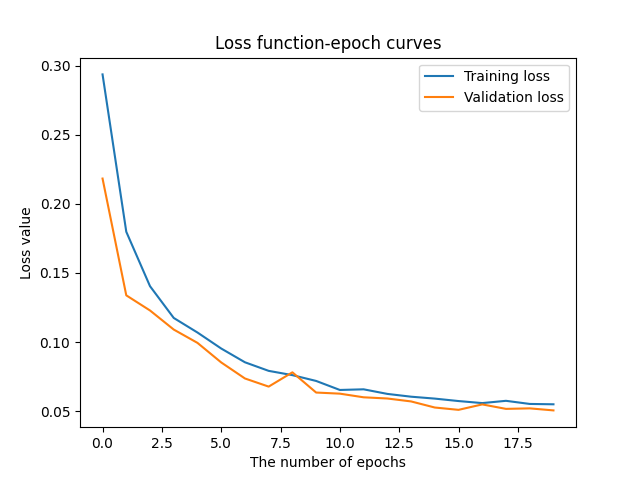
\includegraphics[width=\textwidth]{images/Khanh/Python/Loss_Chart.png}
    \caption{Giá trị Train loss và Val loss}
    \label{fig:loss_chart}
\end{figure}

Sau đó chúng tôi sử dụng tập test để dự đoán và so sánh kết quả dự đoán với dữ liệu thực như hình \ref{fig:test_recycle_actual_prediction} cho mức rác tái chế và hình \ref{fig:test_non_recycle_actual_prediction} cho mức rác không tái chế với kết quả RMSE và MSE cho tập test mức rác tái chế là 97.511 và 86.812, RMSE và MSE cho tập test mức rác không tái chế là 104.531 và 93.270.
\begin{figure}[H]
    \centering
    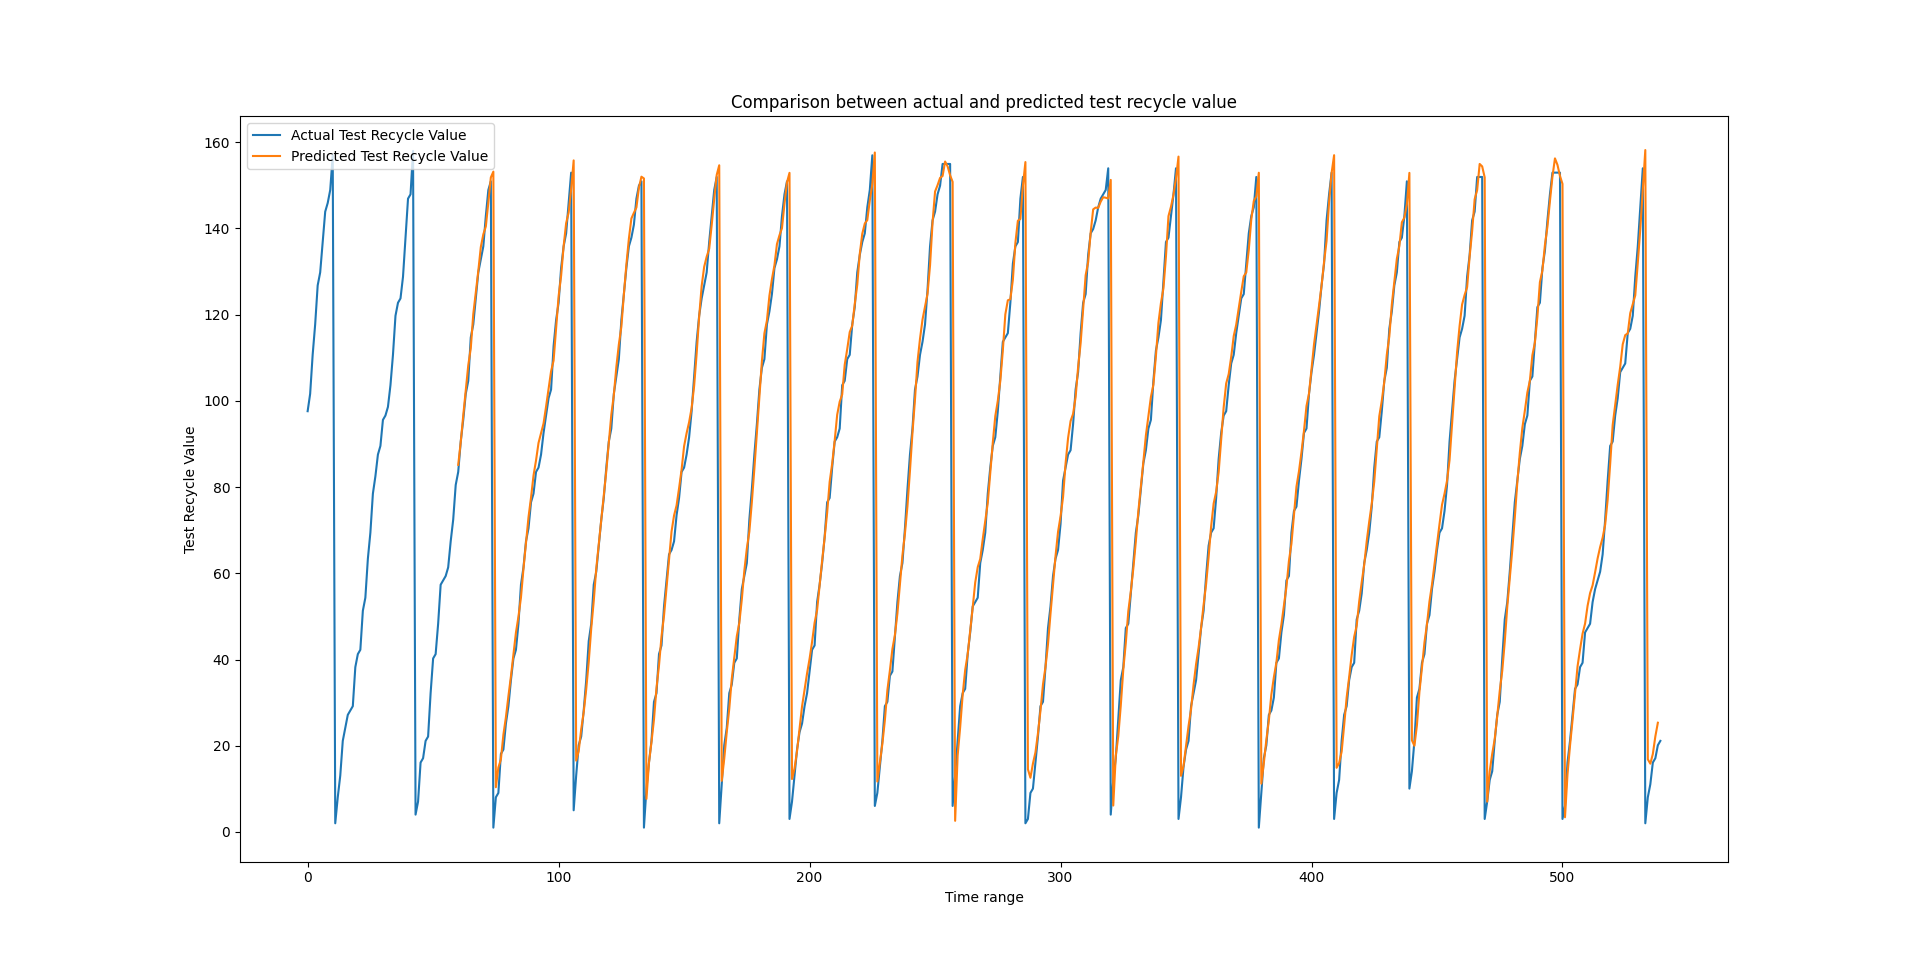
\includegraphics[width=\textwidth]{images/Khanh/Python/Recycle_Test_Chart.png}
    \caption{So sánh actual với predicted của tập test tái chế}
    \label{fig:test_recycle_actual_prediction}
\end{figure}
\begin{figure}[H]
    \centering
    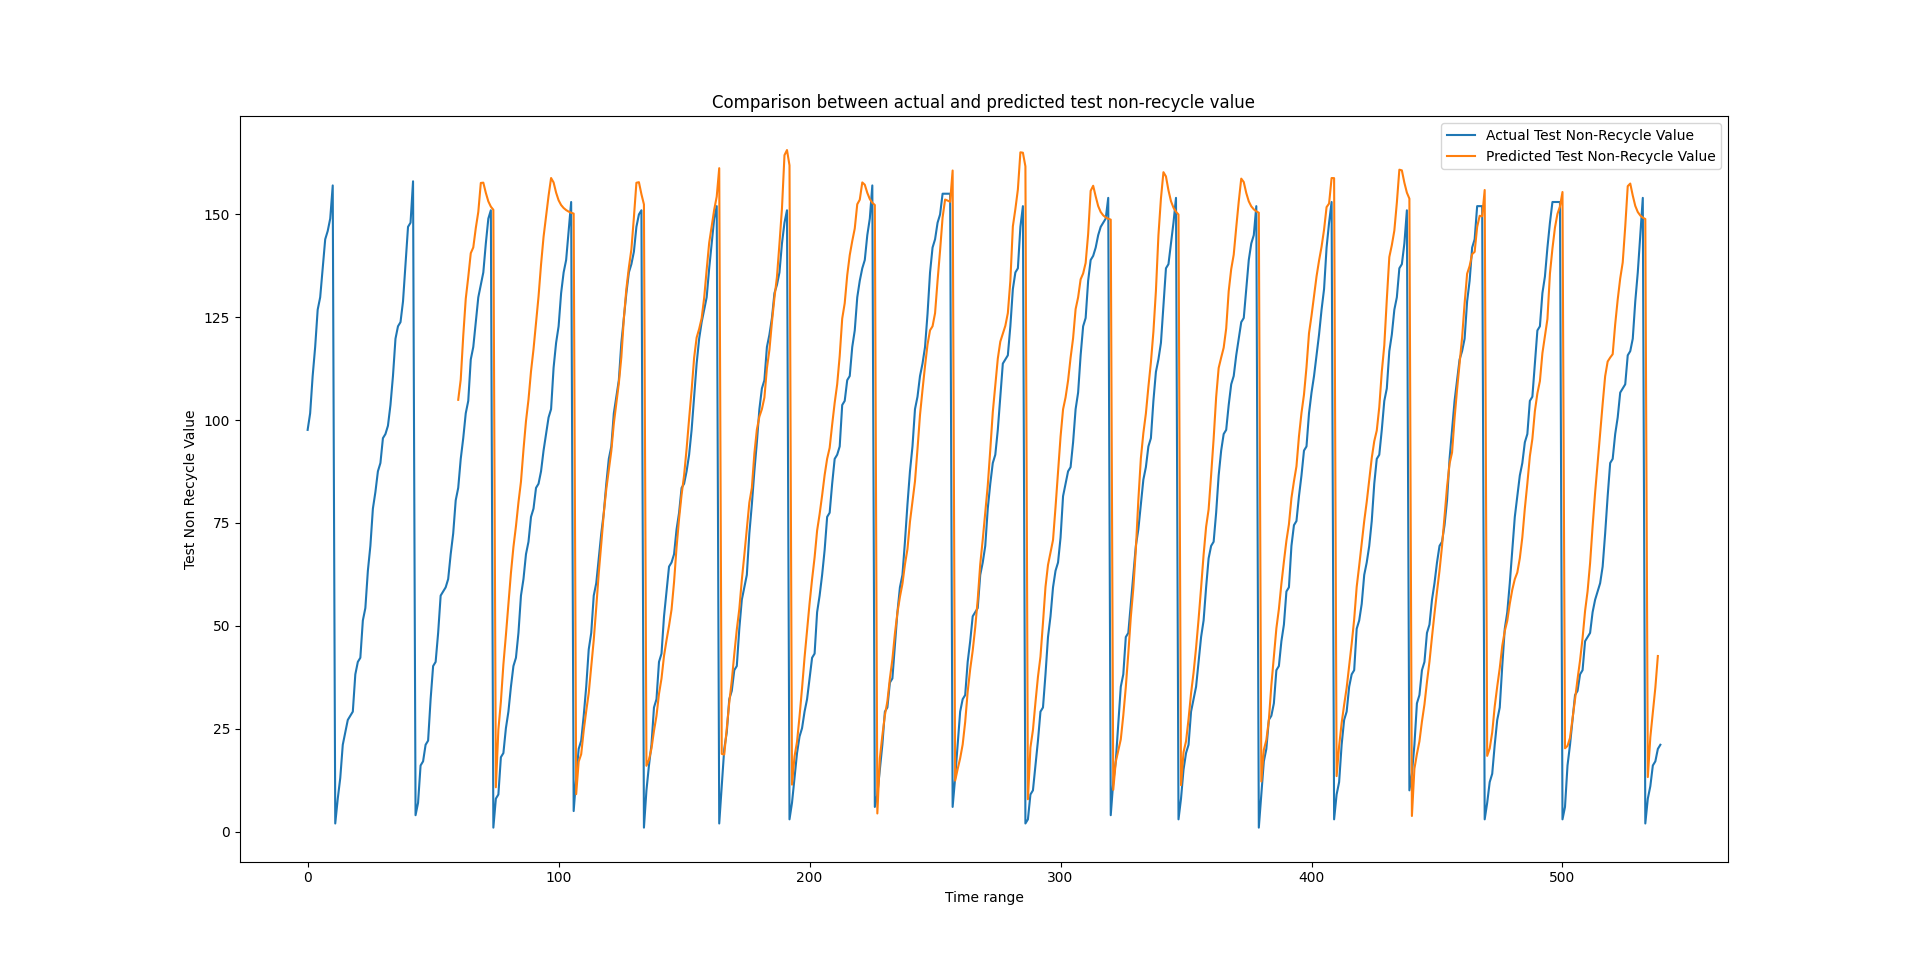
\includegraphics[width=\textwidth]{images/Khanh/Python/Non-Recycle_Test_Chart.png}
    \caption{So sánh actual với predicted của tập test không tái chế}
    \label{fig:test_non_recycle_actual_prediction}
\end{figure}

Ở bước cuối cùng chúng tôi sử dụng model để dự đoán mức rác vào 12 time\_steps (4 tiếng tiếp theo), kết quả hiển thị như hình \ref{fig:final_result}
\begin{figure}[H]
    \centering
    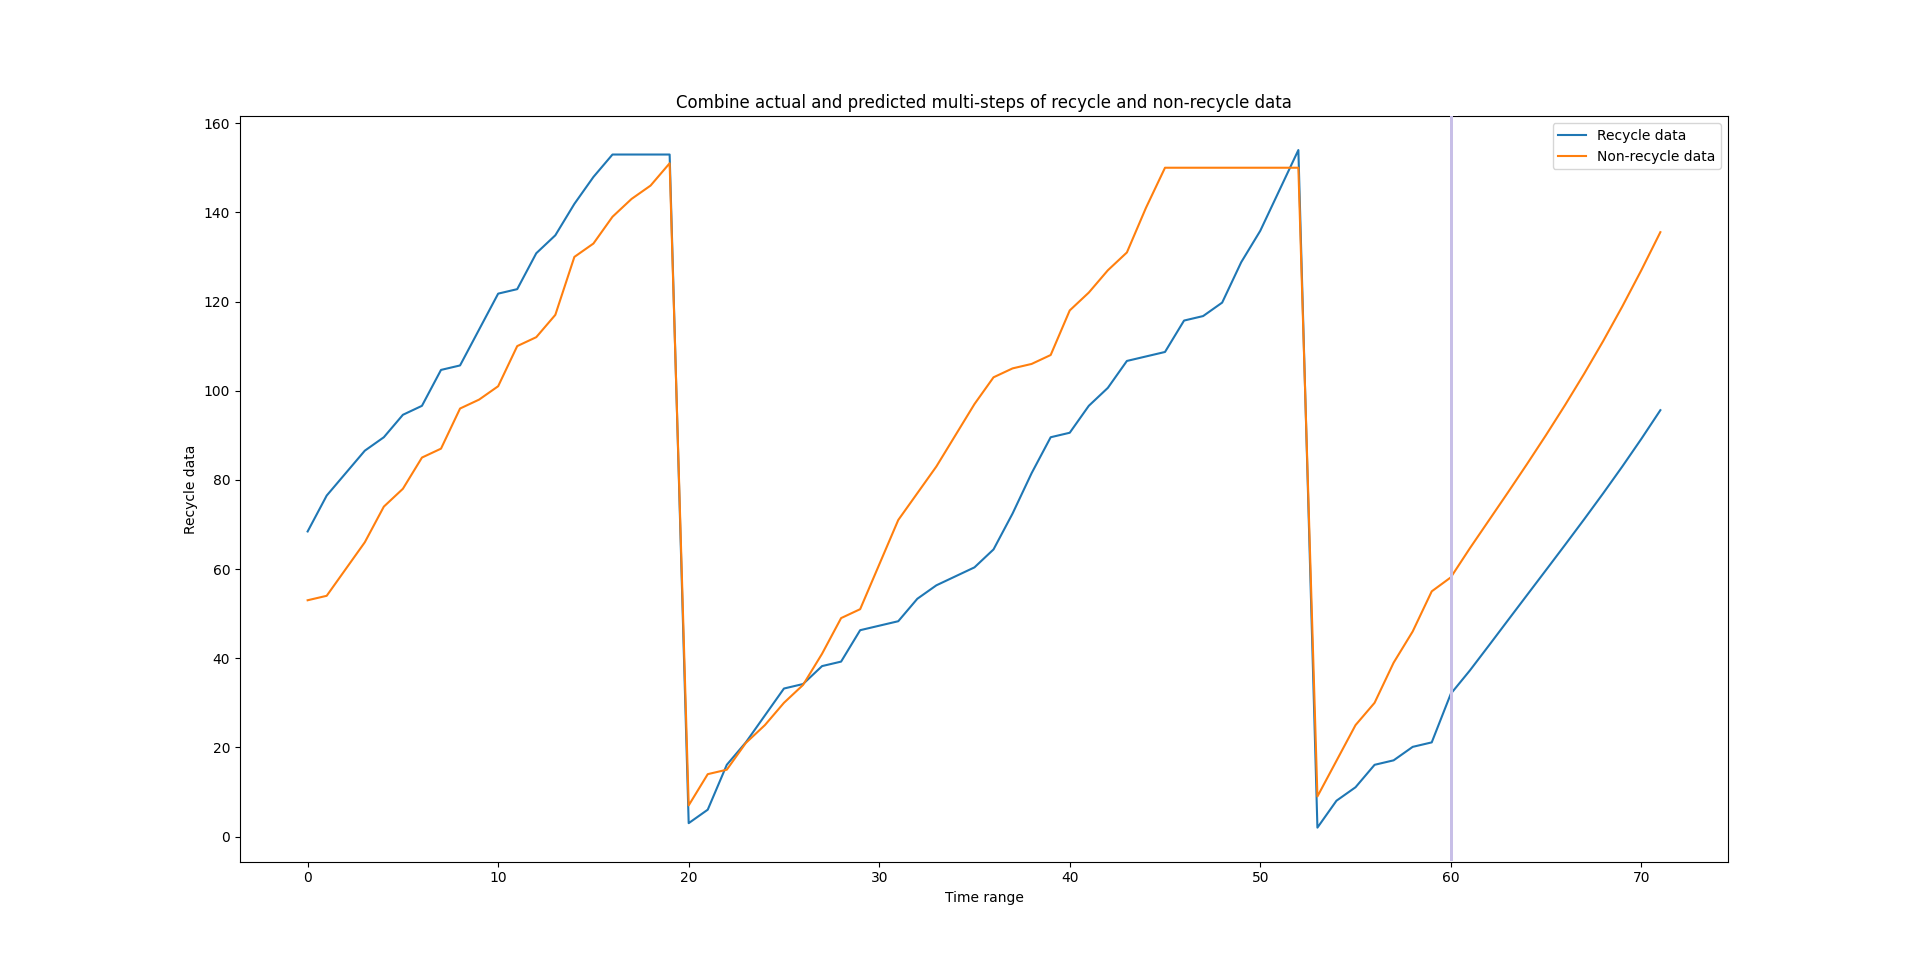
\includegraphics[width=\textwidth]{images/Khanh/Python/Final_results.png}
    \caption{Biểu đồ mức rác tái chế và không tái chế sau 4 tiếng tiếp theo}
    \label{fig:final_result}
\end{figure}

\section{Thingsboard}
\subsection{Giới thiệu tổng quát}
Việc xử lý dữ liệu ở server vẫn chưa đủ, thông tin dữ liệu của thùng rác cần được hiển thị cho cả admin và người dùng quan sát. Vì thế, Thingsboard vừa được sử dụng như một Frontend đáp ứng việc này đồng thời cung cấp một doc cung cấp những API để hỗ trợ đưa thông tin lên giao diện.

Chúng tôi sử dụng bản demo của Thingsboard cho dự án để giảm bớt thời gian cài đặt cho bản Localhost và chi phí cho bản Premium, tuy vậy những tính năng mà bản demo mang lại vẫn đáp ứng đầy đủ những yêu cầu mà dự án cần. 

\subsection{Assets và Devices}
Cả asset và device đều là một thực thể của Thingsboard, ở trong dự án này asset được quy định là thùng rác và device được quy định là cảm biến của thùng rác đó. Những thực thể có thể được tạo thủ công trên giao diện hoặc tự động bằng Thingsboard API, và sẽ được lưu trữ tại database PostgreSQL.

Thingsboard cung cấp 2 tab bao gồm danh sách tất cả asset và device đã tạo như hình \ref{fig:asset_general} và \ref{fig:device_general}.
\begin{figure}[H]
    \centering
    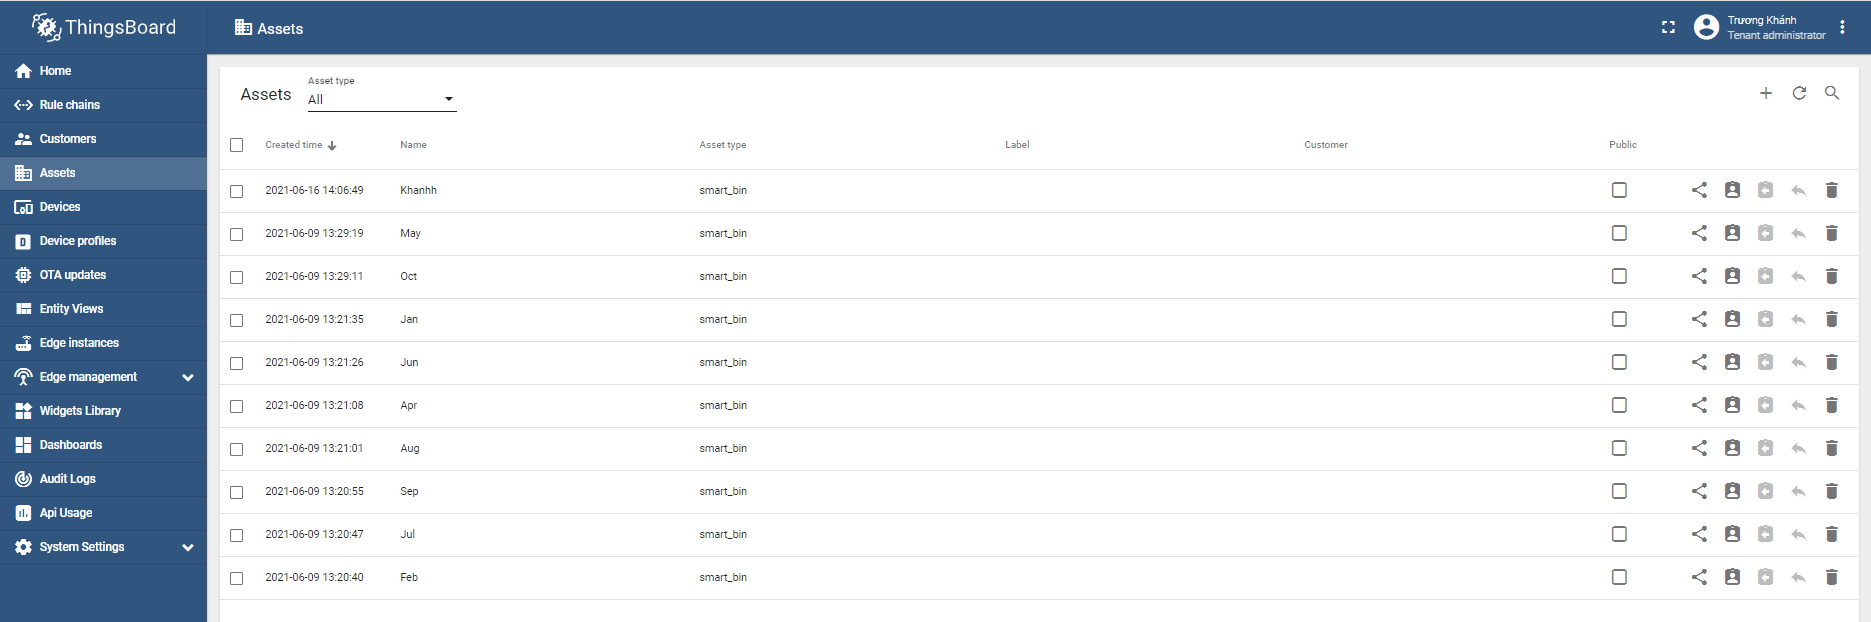
\includegraphics[width=\textwidth]{images/Khanh/Thingsboard/Assets.PNG}
    \caption{Danh sách thùng rác}
    \label{fig:asset_general}
\end{figure}
\begin{figure}[H]
    \centering
    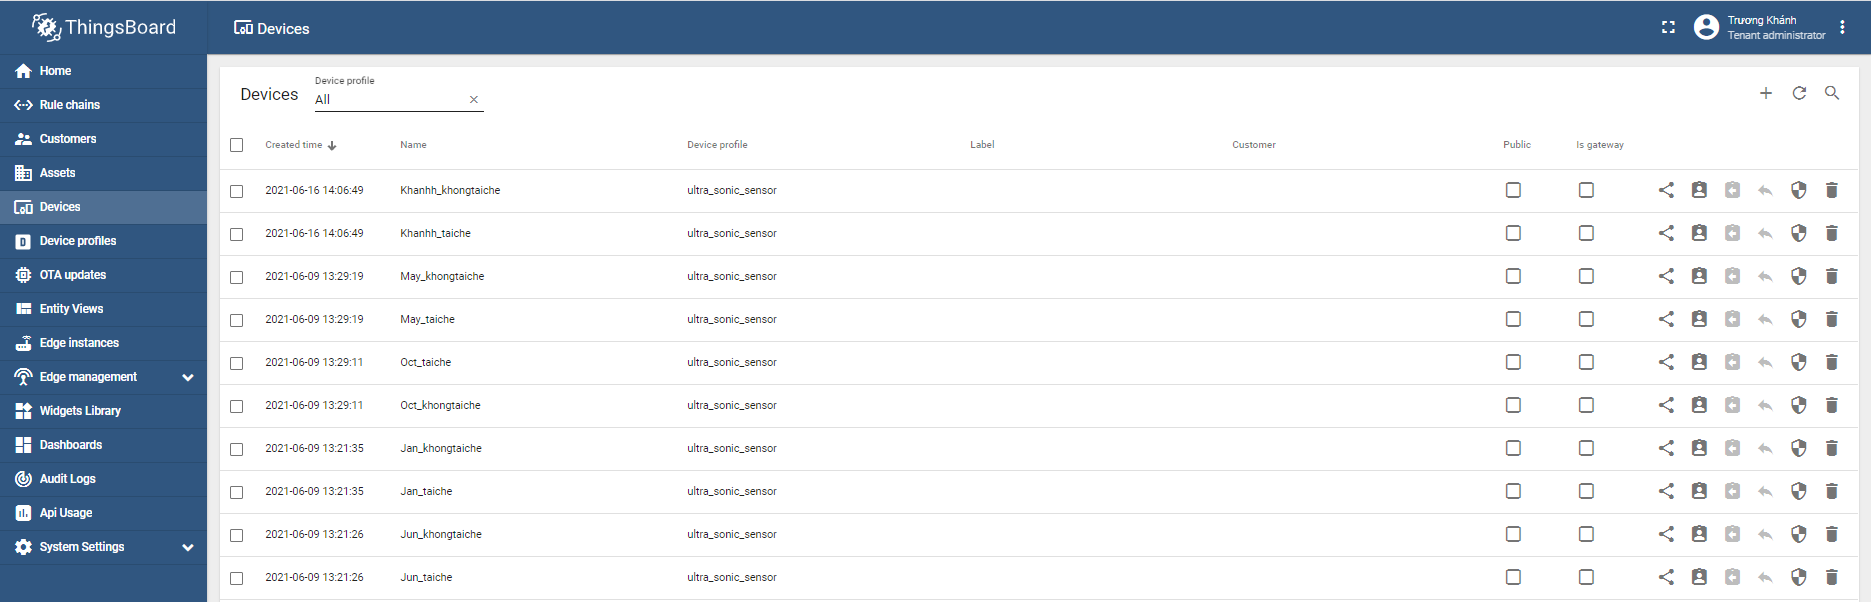
\includegraphics[width=\textwidth]{images/Khanh/Thingsboard/Devices.PNG}
    \caption{Danh sách cảm biến}
    \label{fig:device_general}
\end{figure}

Mỗi thực thể đều có những đặc điểm sau:
\begin{itemize}
    \item Details: chứa thông tin cơ bản của thực thể và một id phân biệt.
    \item Attributes: thuộc tính của thực thế, có thể cập nhật thủ công hoặc tự động thông qua Thingsboard API (hình \ref{fig:asset_attributes}).
    \item Lastest Telemetry: dữ liệu theo thời gian của thực thể, cập nhật thông qua Thingsboard API, mang giá trị gần đây nhất.
    \item Alarms: danh sách các báo động của thực thể.
    \item Events: các sự kiện giúp theo dõi tình trạng của thực thể.
    \item Relations: các mối quan hệ giữa các thực thể với nhau (hình \ref{fig:asset_relation}).
    \item Audit Logs: nhật ký kiểm tra theo dõi hành động người dùng liên quan đến các thực thể.
\end{itemize} 
\begin{figure}[H]
    \centering
    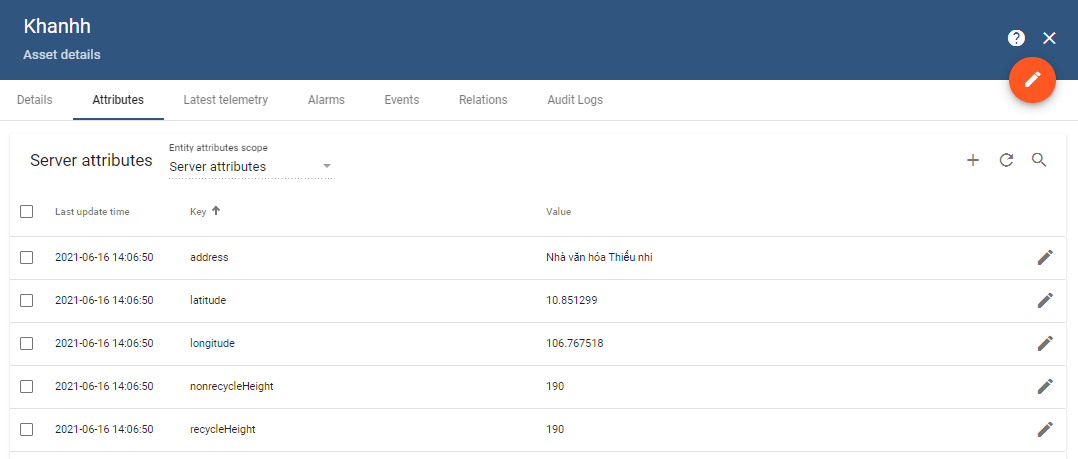
\includegraphics[width=\textwidth]{images/Khanh/Thingsboard/Asset_details.PNG}
    \caption{Thuộc tính thùng rác}
    \label{fig:asset_attributes}
\end{figure}
\begin{figure}[H]
    \centering
    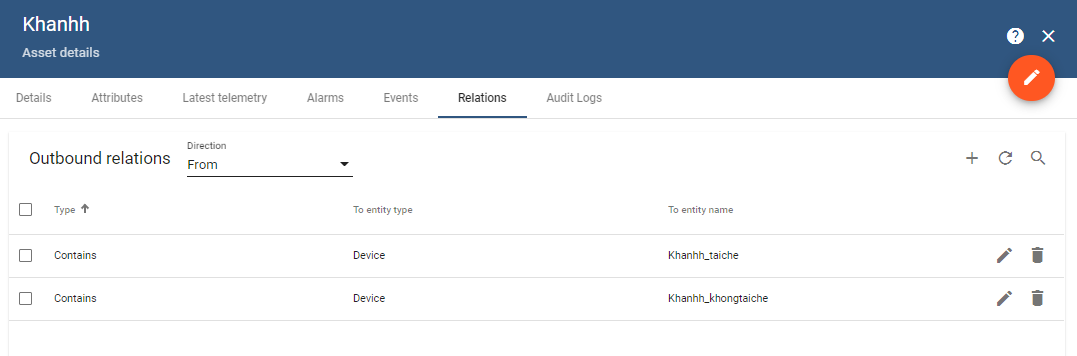
\includegraphics[width=\textwidth]{images/Khanh/Thingsboard/Asset_relation.PNG}
    \caption{Mối quan hệ của thùng rác với cảm biến}
    \label{fig:asset_relation}
\end{figure}

\subsection{Rule Chains}
Rule chains là những khung logic dạng kéo thả (nodes) được nối lại với nhau thành một chuỗi logic (rule chain) dùng để xử lý dữ liệu trực tiếp trên Thingsboard. Những nodes mà Thingsboard cung cấp đều có một chức năng khác nhau và được chia thành từng danh mục theo từng màu.
\begin{itemize}
    \item Filter (vàng): lọc những gói tin tới bằng những điều kiện được lập trình.
    \item Enrichment (xanh lá): thêm thông tin lấy từ thực thể và gắn vào gói tin. 
    \item Transformation (xanh dương): thay đổi thông tin gói tin bằng mã lập trình.
    \item Action (đỏ): tạo những action cho thực thể để xử lý dữ liệu.
    \item External (cam): tương tác với các hệ thống bên ngoài.
    \item Rule Chain (tím): gửi gói tin tới các rule chains khác.
\end{itemize}

Vì dữ liệu lượng rác được gửi từ các cảm biến và thùng rác phải sở hữu và định dạng lại dữ liệu để hiển thị lên biểu đồ đường, nên chúng tôi sử dụng rule chain để lưu dữ liệu vào cảm biến, đổi thực thể sở hữu sang thùng rác và định dạng lại dữ liệu thành chiều cao của thùng. Rule chain được mô tả ở hình \ref{fig:root_chain} và Delta chain \ref{fig:delta_chain}
\begin{figure}[H]
    \centering
    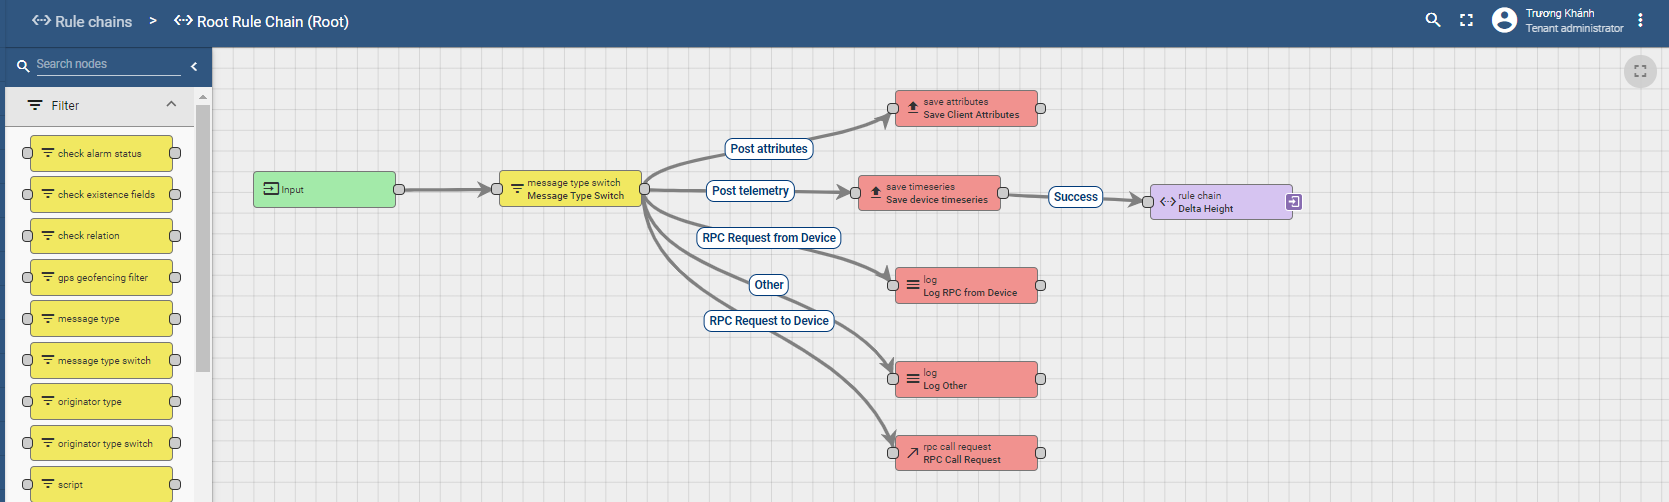
\includegraphics[width=\textwidth]{images/Khanh/Thingsboard/Root_rule_chain.PNG}
    \caption{Root Rule Chain}
    \label{fig:root_chain}
\end{figure}
Root Rule Chain là luồng xử lý chính cho Thingsboard, tất cả gói tin input được gửi từ hệ thống bên ngoài sẽ được lưu vào khung input. Sau đó gói tin sẽ được lọc theo \{MESSAGE\_TYPE\} bằng khung Message Type Switch, những \{MESSAGE\_TYPE\} bao gồm những sự kiện khác nhau liên quan đến thực thể. 

Những thuộc tính của thùng rác sẽ được lọc qua luồng Post attributes và được lưu vào thực thể, còn những dữ liệu thời gian của thùng rác và cảm biến sẽ được lọc qua luồng Post telemetry, được lưu vào thực thể và được gửi qua Delta Rule Chain. Những gói tin thuộc \{MESSAGE\_TYPE\} khác sẽ đi vào luồng khác hoặc được log qua Audit Logs.

\begin{figure}[H]
    \centering
    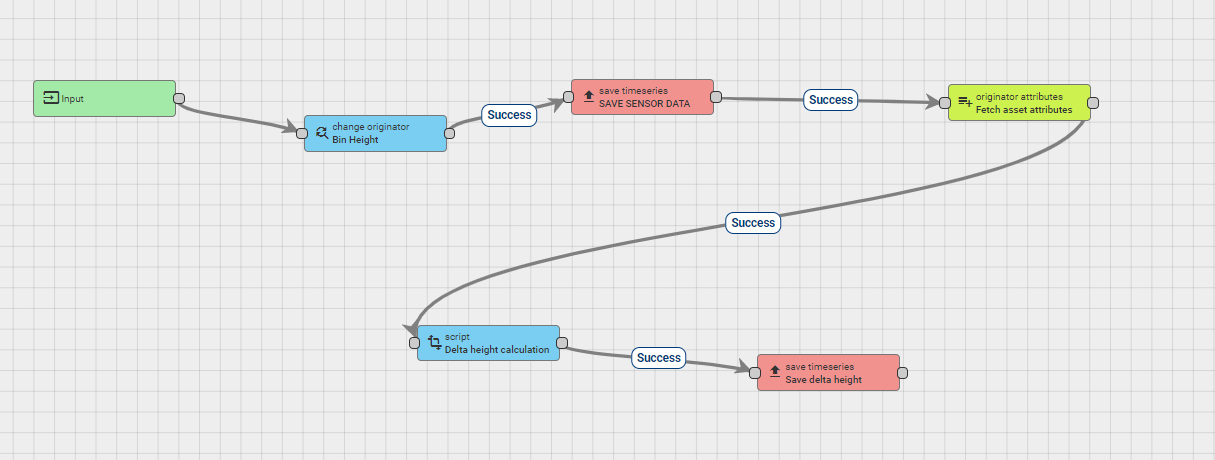
\includegraphics[width=\textwidth]{images/Khanh/Thingsboard/Delta_rule_chain.PNG}
    \caption{Delta-calculation Rule Chain}
    \label{fig:delta_chain}
\end{figure}

Gói tin được lọc từ type Post telemetry sẽ được lưu ở khung input, sau đó dữ liệu mức rác sẽ được chuyển thực thể từ cảm biến sang của thùng rác bằng khung Change originator và được lưu vào thùng rác.

Dữ liệu sau đó được định dạng lại giống chiều cao thùng rác bằng cách lấy chiều cao thùng trừ cho dữ liệu, vì thế sử dụng khung Originator attributes để fetch thuộc tính thực thể và đưa tất cả qua một Transformation script để xử lý logic.

Xử lý dữ liệu mức rác cũng khá đơn giản khi chỉ cần phân chia dữ liệu tái chế và không tái chế và lấy ngăn chiều cao trừ cho dữ liệu, kết quả gửi qua khung Save timeseries để lưu dữ liệu vào thùng rác.

\subsection{Dashboard}
Dashboard là khung màn hình hiển thị chính của Thingsboard, được tạo bởi các widget hỗ trợ sẵn (biểu đồ, bản đồ, bảng, input tương tác, alarms, ...), hỗ trợ hiển thị, tương tác và trực quan hóa dữ liệu theo nhiều cách. 

Dashboard cho phép chúng ta tạo ra nhiều các dashboard khác, trong một dashboard, ta có thể có nhiều state và action event để di chuyển giữa các state, nhiều Entity aliases để phân biệt và gom cụm các thực thể lại với nhau và thêm vào các widget để lấy dữ liệu dễ dàng hơn.

Ở trang dashboard chính, chúng tôi cho hiển thị bản đồ hiện tất cả những thùng rác được tạo như hình \ref{fig:dashboard_map} và một danh sách các thùng rác gồm các thuộc tính của nó như hình \ref{fig:dashboard_asset_list}

\begin{figure}[H]
    \centering
    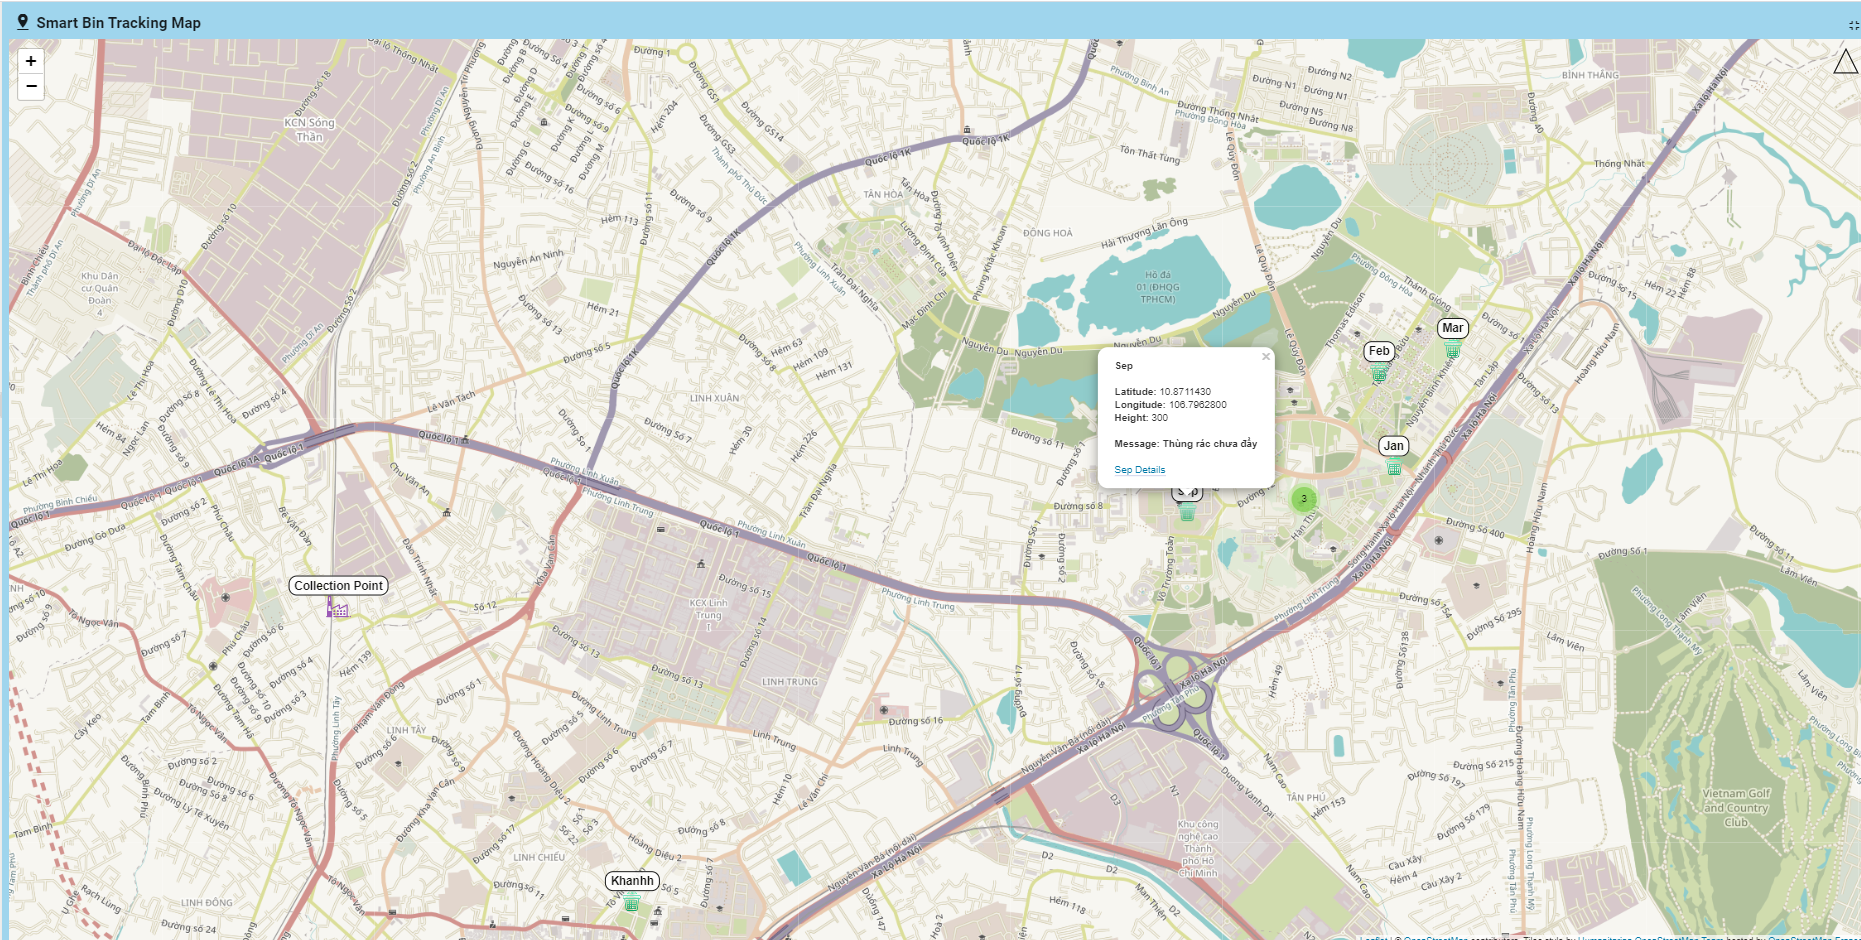
\includegraphics[width=\textwidth]{images/Khanh/Thingsboard/Dashboard_map.PNG}
    \caption{Bản đồ theo dõi vị trí thùng rác}
    \label{fig:dashboard_map}
\end{figure}
Bản đồ hiển thị tất cả các thùng rác và địa điểm thu gom rác, được phân biệt bằng icon khác nhau và các thùng rác được clustering để gom cụm từng vùng. Với mỗi thùng rác, khi nhận được trạng thái đầy sẽ chuyển thành màu đỏ để dễ nhận biết. Ngoài ra, mỗi thùng rác còn có tooltip hiện tên, tọa độ, chiều cao, chuỗi thông báo và một đường link dẫn đến state chi tiết của thùng rác. 

Bản đồ này cũng tích hợp tính năng Polygon để vẽ tuyến đường, có thể thích ứng với chức năng tìm đường tối ưu nhất từ nơi gom rác đến tất cả thùng rác đầy như hình \ref{fig:map_optimization}.
\begin{figure}[H]
    \centering
    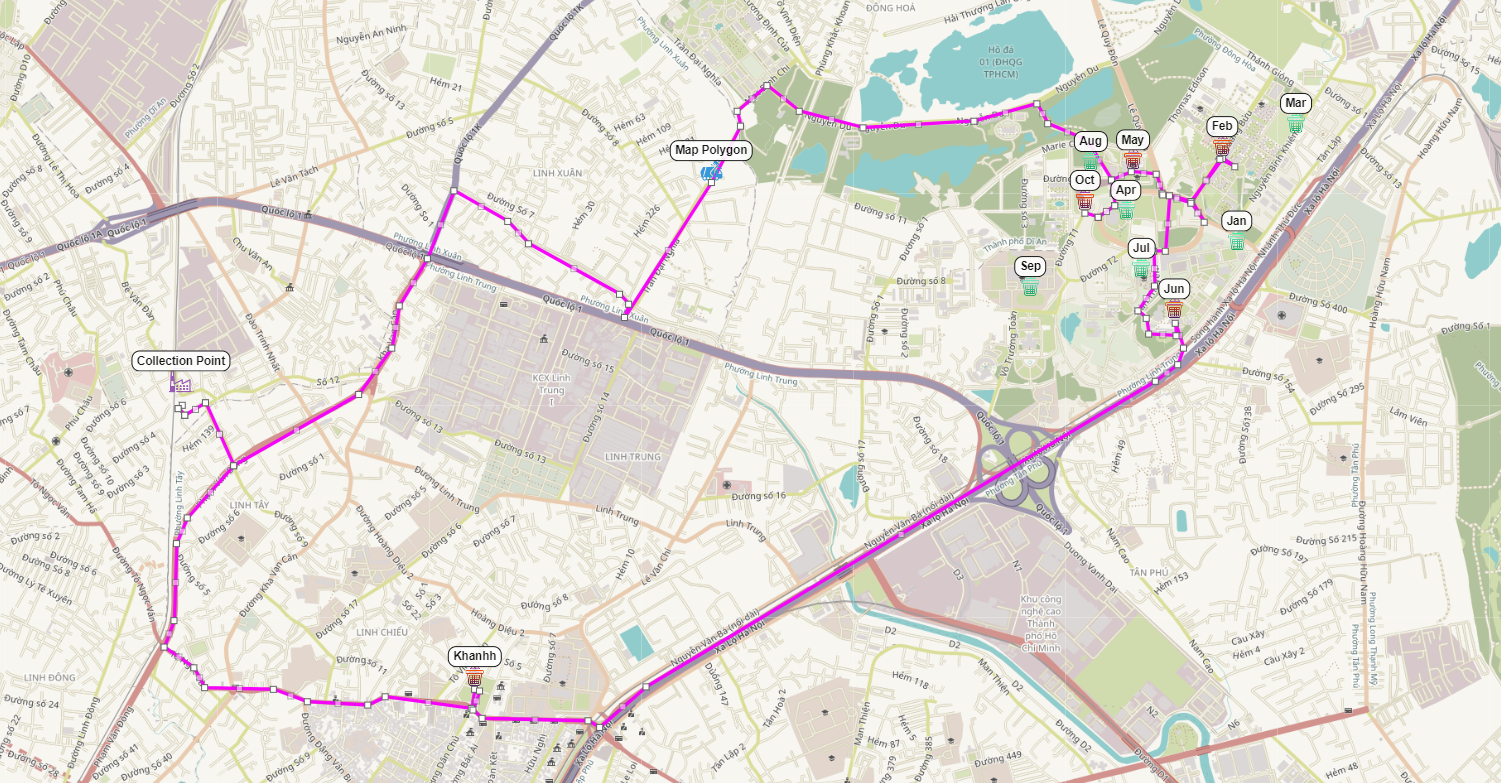
\includegraphics[width=\textwidth]{images/Khanh/Thingsboard/Road_optimization.PNG}
    \caption{Polygon các tọa độ đường đi trên bản đồ}
    \label{fig:map_optimization}
\end{figure}

\begin{figure}[H]
    \centering
    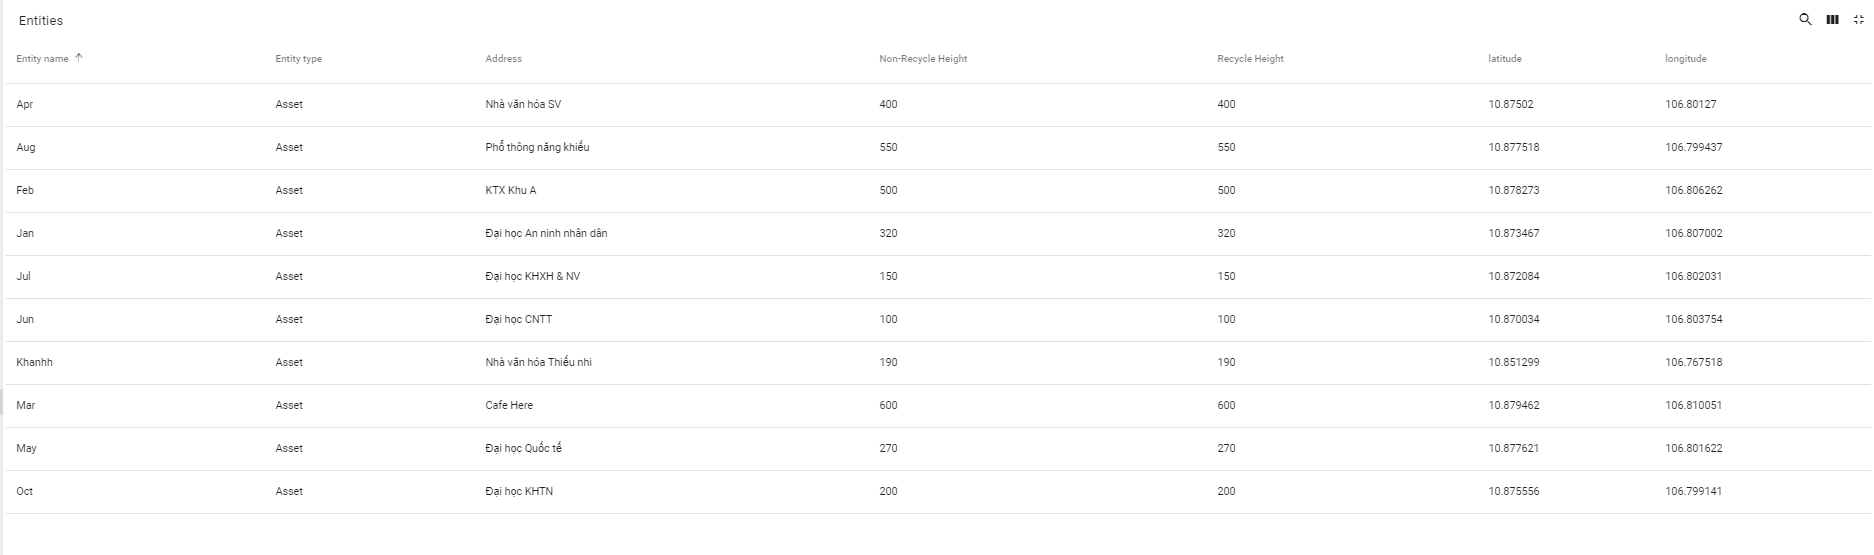
\includegraphics[width=\textwidth]{images/Khanh/Thingsboard/Dashboard_list.PNG}
    \caption{Danh sách thùng rác hiện có}
    \label{fig:dashboard_asset_list}
\end{figure}
Danh sách các thùng rác bao gồm tên, loại, địa chỉ, tọa độ và chiều cao hai ngăn của thùng, mỗi thùng rác được gắn sự kiện event khi nhấn vào thì sẽ chuyển qua state dashboard khác, cụ thể là state hiển thị dữ liệu của thùng rác và các cảm biến của nó.

Ở state dashboard chi tiết từng thùng rác, giao diện được bố trí như hình \ref{fig:bin_detail}, với một biểu đồ đường hiển thị mức rác tái chế và không tái chế của thùng, ở dưới bên trái là danh sách các cảm biến của thùng rác cùng với dữ liệu của cảm biến, còn ở bên phải là bảng thông báo tình trạng của thùng rác bao gồm tình trạng chưa đầy, đã đầy hoặc dự tính đã đầy trong một khoảng thời gian tới. 
\begin{figure}[H]
    \centering
    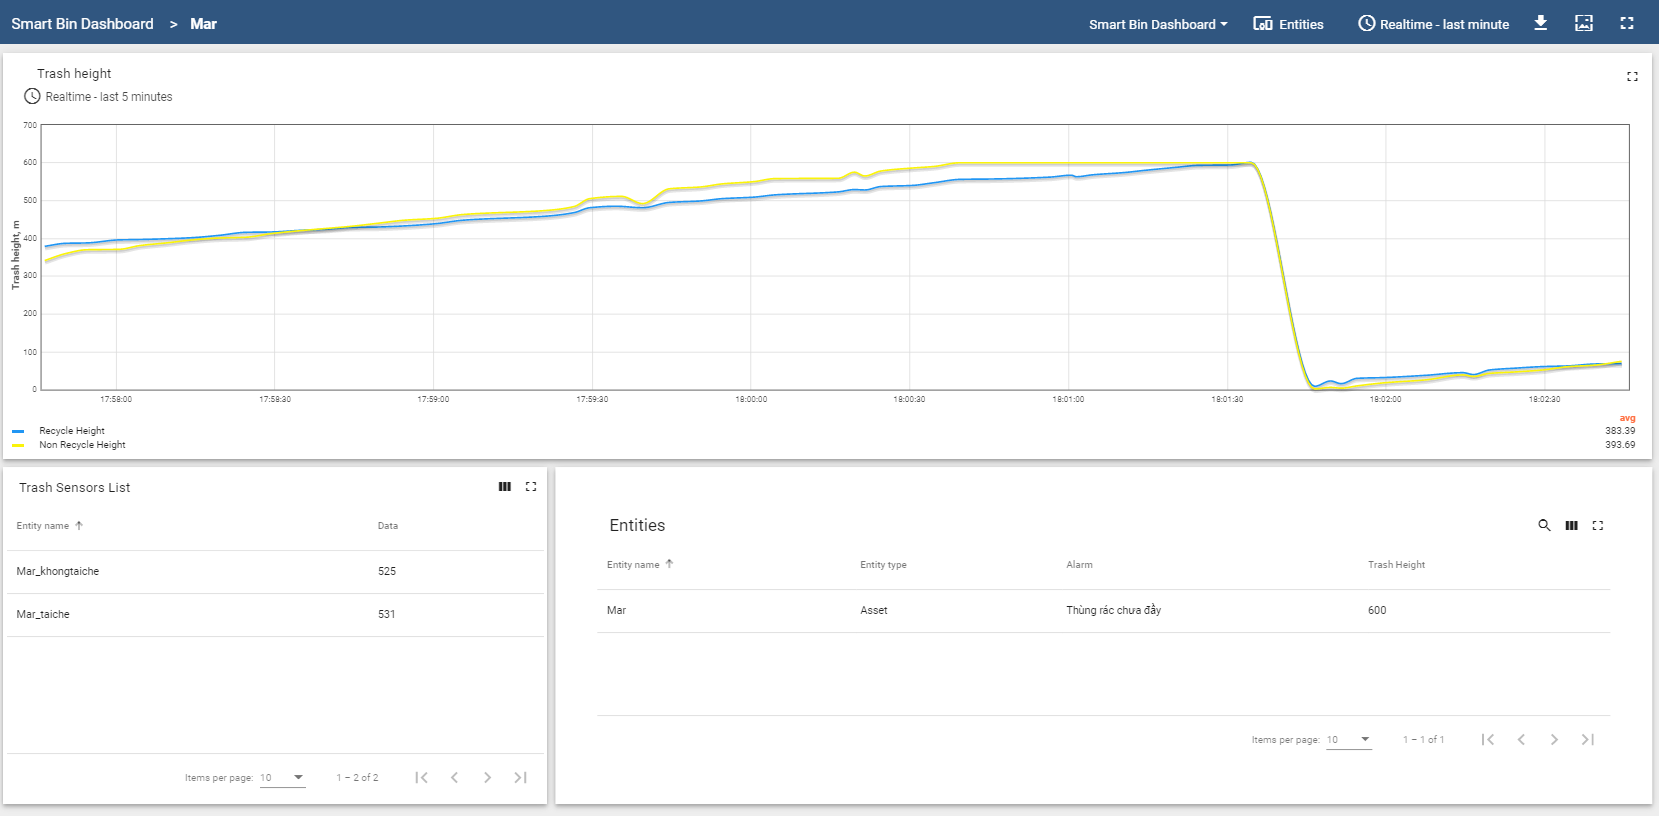
\includegraphics[width=\textwidth]{images/Khanh/Thingsboard/Bin_detail.PNG}
    \caption{Giao diện chi tiết của thùng rác thông minh}
    \label{fig:bin_detail}
\end{figure}

Khi nhấn vào mỗi cảm biến của thùng rác, dashboard sẽ chuyển sang state mới hiển thị biểu đồ dữ liệu của cảm biến theo thời gian như hình \ref{fig:sensor_detail}.
\begin{figure}[H]
    \centering
    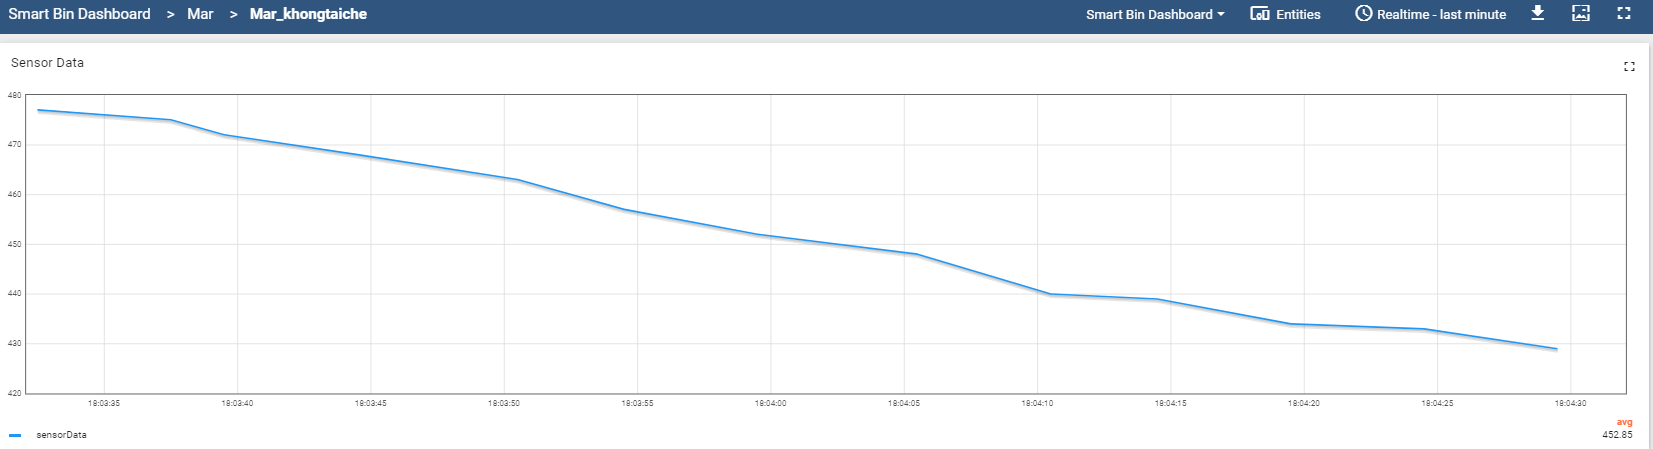
\includegraphics[width=\textwidth]{images/Khanh/Thingsboard/Sensor_detail.PNG}
    \caption{Biểu đồ thể hiện dữ liệu của cảm biến}
    \label{fig:sensor_detail}
\end{figure}